\graphicspath{{included-papers-tex/paper-11/}}

%\includedPaper{\textsc{paper vi - designer modeling through design style clustering}}{\textsc{paper vi - designer modeling through design style clustering}}{Alberto Alvarez, Jose Font, and Julian Togelius}

\includedPaper{\textsc{paper xi - Story Designer: \\ Towards a Mixed-Initiative Tool to Create Narrative Structures}}{Paper XI - Story Designer: Towards a Mixed-Initiative Tool to Create Narrative Structures}{Alberto Alvarez, Jose Font, and Julian Togelius}

\normalfont
\textbf{\textsc{ABSTRACT}}

Narratives are a predominant part of games, and their design poses challenges when identifying, encoding, interpreting, evaluating, and generating them. One way to address this would be to approach narrative design in a more abstract layer, such as narrative structures. This paper presents Story Designer, a mixed-initiative co-creative narrative structure tool built on top of the Evolutionary Dungeon Designer (EDD) that uses tropes, narrative conventions found across many media types, to design these structures. Story Designer uses tropes as building blocks for narrative designers to compose complete narrative structures by interconnecting them in graph structures called narrative graphs. Our mixed-initiative approach lets designers manually create their narrative graphs and feeds an underlying evolutionary algorithm with those, creating quality-diverse suggestions using MAP-Elites. Suggestions are visually represented for designers to compare and evaluate and can then be incorporated into the design for further manual editions. At the same time, we use the levels designed within EDD as constraints for the narrative structure, intertwining both level design and narrative. We evaluate the impact of these constraints and the system's adaptability and expressiveness, resulting in a potential tool to create narrative structures combining level design aspects with narrative.

\textbf{\textsc{PUBLISHED IN}}

Proceedings of the Foundations of Digital Games (FDG), ACM, 2022.

\section*{STORY DESIGNER: TOWARDS \\ A MIXED-INITIATIVE TOOL TO CREATE NARRATIVE STRUCTURES}

\subsection{Introduction}

% \begin{itemize}
%     \item The paper will have two main contributions:
%     \begin{itemize}
%         \item The implementation of Tropetwist into a Mixed-Initiative system (Story Designer). With that, of course it comes all the new workflow/GUI, how the design works, and how that works with MAP-Elites, etc.
%         \item The new dimensions to be used
%         \item The connection between the Level design and the Story Struct design. The main thing here is that the information from the level is extracted and that constraints what can be designed and MAP-Elites. IC MAP-Elites uses these constraints to identify what individuals are feasible and unfeasible.
%     \end{itemize}
% \end{itemize}

% \begin{itemize}
%     \item Talk about the combination between level (space) and narrative
%     \item What is Story Designer and what can it be used for
%     \item what is the point of the system? give an example.
%     \item what did we do in the paper?/contributions!
% \end{itemize}



%julian The intro in its current state is light on motivation and heavy on references to narrative theory; for someone who is not already well-read on this theory, it is not very understandable.
%Agree, it should be adjusted to motivate better.



%coherently intertwines
Games are multifaceted content that intertwines gameplay, mechanics, audio, level, graphics, and narrative facets~\citepeleventh{p11liapis_orchestrating_2019}. Narrative has been linked as a key facet to connect different components in games such as level design~\citepeleventh{p11kishino_hunt_2005}, and to create meaningful interactions with depth and context~\citepeleventh{p11ashmore_quest_2007,p11kybartas_quinn_survey_2017}. Thus, narrative in games has been a focus of study~\citepeleventh{p11aarseth_narrative_2012,p11eladhari_interweaving_2014,p11yu_what_2020} and its generation has been approached in different ways and with different techniques~\citepeleventh{p11smith_situating_2011,p11ammanabrolu_story_2020,p11green_data_2018,p11tambwekar_controllable_2019,p11alvarez_questgram_2021}.

Patterns have been a common approach to narrative and other facets. The focus then has been on extracting common narrative aspects to ease the identification, encoding, and generation of narrative in different forms~\citepeleventh{p11doran_prototype_2011,p11alvarez_tropetwist_2022,p11trenton_quest_2010,p11treanor_ai-based_2015,p11rouse_sketching_2018,p11breault_let_2021}. However, it remains a challenge to define certain narrative aspects more aligned with the structure and overarching goals of the game given what type of content is generated, as well as using these to design and compare among games. One approach would be to change the abstraction level at which the narrative is designed. Instead of focusing on the details, quests, or plot, one could focus on the structure. Narrative structures can be used to describe how a story is to be developed, as argued by Barthes~\citepeleventh{p11barthes_introduction_1966}, and to create an abstract representation that reveals common structures among them, such as Propp's 31 ``narremes" ~\citepeleventh{p11propp_morphology_1975}. One approach to generate narrative structures is TropeTwist~\citepeleventh{p11alvarez_tropetwist_2022}, which uses tropes, narrative conventions found across many media types~\citepeleventh{p11lewis_governing_2018,p11garcia-sanchez_simpsons_2021}, as patterns to design these structures.

This paper presents Story Designer, a mixed-initiative co-creative (MI-CC) narrative structure tool built on top of the Evolutionary Dungeon Designer (EDD) using the TropeTwist system. Story Designer uses tropes as building blocks for designers to compose complete narrative structures by interconnecting them in graph structures called narrative graphs. Story Designer lets designers create narrative graphs and assist them with a suggestion grid that uses the Interactive Constrained MAP-Elites (IC MAP-Elites)~\citepeleventh{p11alvarez_interactive_2020}. By having an MI-CC system to design narrative structures, designers could ideate and prototype their structures while the system adapts and suggest novel narratives, making use of patterns, optimizing coherence, and situating the narrative structures along dimensions of interest for designers. At the same time, IC MAP-Elites can take advantage and use the designer's structure as a proxy to evaluate subjective characteristics such as interestingness, which has been the subject of several studies~\citepeleventh{p11perez_model_2013,p11lankoski_models_2013,p11rowe_storyeval_2009}.

%to generate variations focusing on the graph's coherence and the dimensions that the designer might be interested. 

As Story Designer is implemented in EDD and based on the link between level design and narrative, we make use of the designed dungeon to create constraints over the narrative generation, effectively intertwining both facets. We assess Story Designer with four controlled and simulated experiments, three premade structures of different games, and one step by step design that showcasze the possibilities within the system. All experiments were tested with and without level design constraints and using a pair of dimensions and all dimensions during the search. Our results indicate that IC MAP-Elites have consistency and stability in generating content and that delimiting the search space with additional level constraints, while limiting the diversity and generation of complex structures, guides better the search.

\begin{figure*}[t]
\centering
  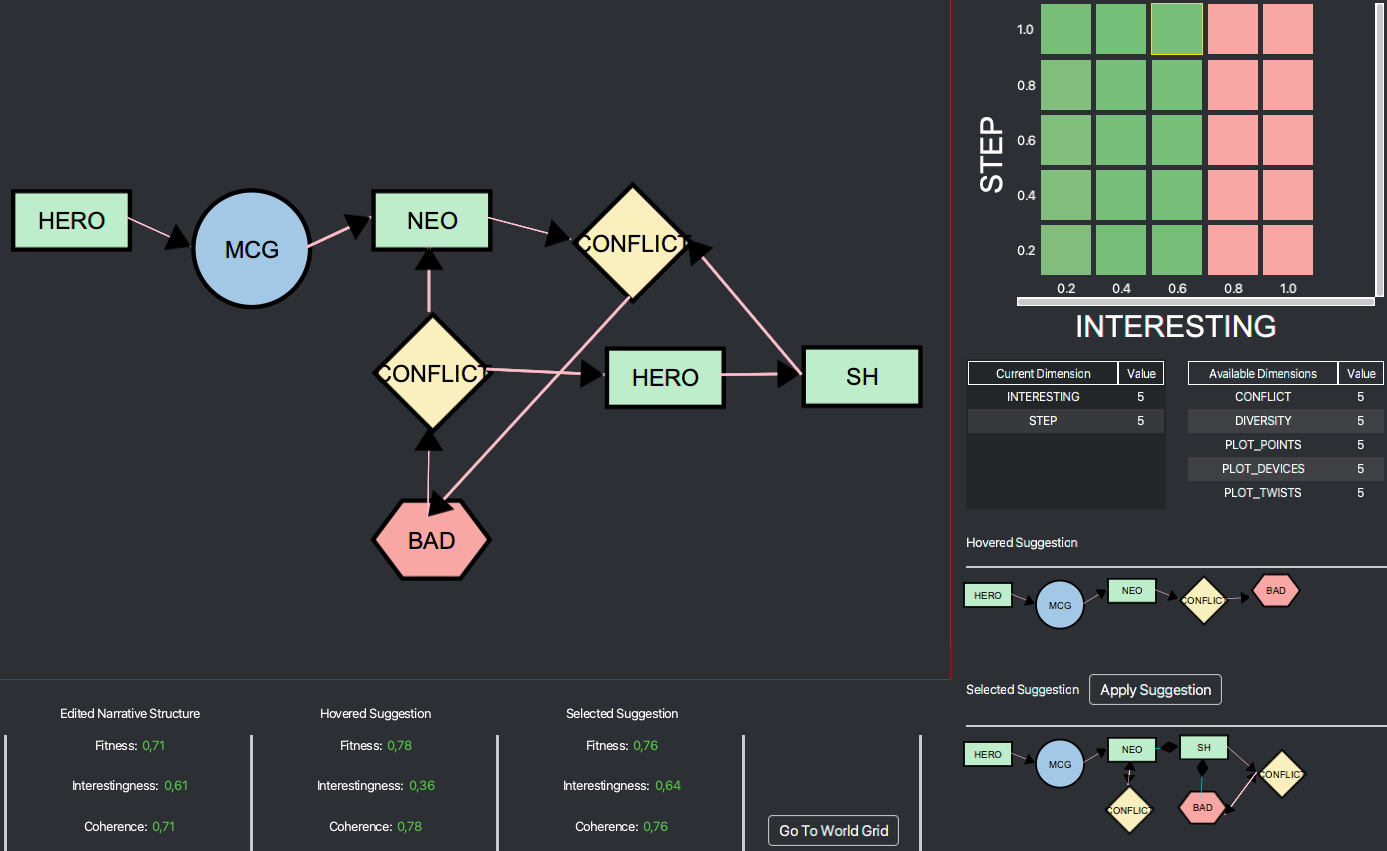
\includegraphics[width=\textwidth]{figures/current_GUI_fixed.png}
\caption{The Story Designer screen in the Evolutionary Dungeon Designer. In the center, there is the main narrative graph being edited by the designer. to the right, the suggestion grid using the Interactive Constrained MAP-Elites (IC MAP-Elites), the possible dimensions to be used, and two inspected suggestions. At the bottom, Story Designer presents some extra information regarding fitness, interestingness, and coherence, for the designer's convenience.}
    \label{fig:story-screen}
\end{figure*}
\subsection{Background}

% Machine Learning (ML) has gained an increased interest from game researchers, achieving remarkable success on training AI agents for very popular games, such as AlphaStar on Starcraft 2 \citepsixth{p6alphastarblog} and OpenAI Five on Dota 2 \citepsixth{p6berner2019dota}. Its combination with PCG has led to the raise of  Procedural Content Generation via Machine Learning (PCGML), defined as the generation of game content by models that have been trained on existing game content \citepsixth{p6summerville2018procedural}, with applications to autonomous content generation, content repair, content critique, data compression, and mixed-initiative design. 

Player modeling, the ability to recognize general socio-emotional
and cognitive/behavioral patterns in players \citepsixth{p6thawonmas2019artificial}, has been appointed by the game research community as an essential process in many aspects of game development, such as designing of new game features, driving marketing and profitability analyses, or as a means to improve PCG and game content adaptation. Player modeling frequently relies on data-driven and ML approaches to create such models out of several sorts of user-generated gameplay data \citepsixth{p6liapismodellingquality19,p6melhart2020feel,p6Drachen2009-playerModellingTombRaider,p6Holmgard2019-proceduralPersonas,p6Melhart2019-ModellingMotivation}.

Using player data from \textit{Iconoscope}, a freeform creation game for visually depicting semantic concepts, Liapis et al. trained and compared several ML algorithms by their ability to predict the appeal of an icon from its visual appearance~\citepsixth{p6liapismodellingquality19}. Furthermore, Alvarez and Vozaru explored personality-driven agents based on individuals' personalities using the \textit{cibernetic big five model}, evaluating how observers judged and perceived agents using data from their personality test when encountering multiple situations~\citepsixth{p6Alvoz2019-PersonalityDriven}. 

%  using Bartle's player archetypes~\citepsixth{p6bartle1996-taxonomy}

Moreover, training models on gameplay data from \textit{Tom Clancy's The Division} has also been used to model, and therefore find predictors of player motivation \citepsixth{p6Melhart2019-ModellingMotivation}, which renders a very valuable tool for understanding the psychological effects of gameplay. Former research followed a similar approach in \textit{Tomb Raider Underworld}, training player models on high-level playing behavior data, identifying four types of players as behavior clusters, which provide relevant information for game testing and mechanic design \citepsixth{p6Drachen2009-playerModellingTombRaider}. Melhart et al. take these approaches one step further by modeling a user's \textit{Theory of Mind} in a human-game agent scenario \citepsixth{p6melhart2020feel}, finding that players' perception of an agent's frustration is more a cognitive process than an affective response. %Alvarez and Vozaru did similar work, exploring personality-driven agents based on individuals' personality using the \textit{cibernetic big five model}, evaluating how observers judged and perceived agents using data from their personality test when encountering multiple situations~\citepsixth{p6Alvoz2019-PersonalityDriven}.

%Alvarez and Vozaru did similar work, exploring personality-driven agents based on individuals' personality using the \textit{cibernetic big five model}, which treats personality-driven agents as goal-based entitites, evaluating how observers judged and perceived agents using data from their personality test when encountering multiple situations~\citepsixth{p6Alvoz2019-PersonalityDriven}.
%modeling individual agents based 

\subsubsection{The Player is the Designer}

Mixed-initiative co-creativity (MI-CC)~\citepsixth{p6yannakakis2014micc}, is the subset of PCG algorithms where human users and AI systems engage in a constant mutual inspiration loop towards the creation of game content \citepsixth{p6charity2020baba,p6machado2019pitako,p6shaker2013ropossum,p6smith_tanagra:_2011,p6liapis_generating_2013}. Understanding player behavior and experience, as well as predicting the player's motivation and intention is key for mixed-initiative creative tools while aiming to offer in real-time user-tailored procedurally generated content. Nevertheless, the player is the designer in MI-CC, and gameplay data is replaced by a compilation of designer-user actions and AI model reactions over time while both user and model are engaged in a mutually inspired creative process. A fluent MI-CC loop should provide good human understanding and interpretation of the system, as well as accurate user behavior modelling by the system, capable of projecting the user's subsequent design decisions \citepsixth{p6ComptonPhD}. 

%Similar to user or player modeling, designer modeling for content creation tools (CAD and MI-CC tools) was suggested by Liapis et al~\citepsixth{p6Liapis2013-designerModel}, where it is proposed the use of designers models that capture their styles, preferences, goals, intentions, and interaction processes. In their work, they suggest methods, indications, and advice on how each part can be model to be integrated into a holistic designer model, and how each game facet can use and benefit from designer modeling. Moreover, in \citepsixth{p6Liapis2014-designerModelImpl} the same authors discuss their implementation of designer modeling and the challenges of integrating all together in their MI-CC tool, Sentient Sketchbook, which had a positive outcome on the adaptation of the tool towards individual “artificial” users.

Shifting towards a designer-centric perspective means that besides focusing on player modeling, it is necessary to focus on modeling the designers. Liapis et al.~\citepsixth{p6Liapis2013-designerModel,p6Liapis2014-designerModelImpl} introduced designer modeling for personalized experiences when using computer-aided design tools, with a focus on the integration of such in automatized and mixed-initiative content creation. The focus is on capturing the designer's style, preferences, goals, intentions, and iterative design process to create representative models of designers. Through these models, designer's and their design process could be understood in-depth, enabling adaptive experiences, further reducing their workload and fostering their creativity. 

%\citepsixth{p6charity2020baba,machado2019pitako,shaker2013ropossum,smith_tanagra:_2011,Machado2017,liapis_generating_2013}. 

% Moreover, goal 13 in the guidelines for Human-AI interaction \citepsixth{p6amershi2019guidelines} highlights the importance of learning from user behavior and personalize the user’s experience by learning from their actions over time. 


%Nourani et al.~\citepsixth{p6Nourani2019-meaningfulExplanations}, who discuss the effects of meaningful and meaningless explanations to users of an AI interactive systems, and their results demonstrates that when an explanation is not aligned with human-logic it significantly affect the user's perception of the system and it's usability is hindered.

Furthermore, lack of transparency is a key impediment for the advancement of human-AI systems, being eXplainable AI (XAI) an emergent research field that holds substantial promise for improving model explainability while maintaining high-performance levels~\citepsixth{p6adadi2018peeking,Doshi-Velez2018}. However, explanations should be aligned with the users' understanding to don't hinder the usability of systems, as demonstrated by Nourani et al.~\citepsixth{p6Nourani2019-meaningfulExplanations}, who discuss the effects of meaningful and meaningless explanations to users of an AI interactive systems.

Zhu et al.~\citepsixth{p6Zhu2018-XAIDesignersMICC} proposed the field of eXplainable AI for Designers (XAID) as a human-centered perspective on MI-CC tools. This work discusses three principles of mixed-initiative, \emph{explainability}, \emph{initiative}, and \emph{domain overlap}, where the latter focuses on the study of the overlapping creative tasks between game designers and black-box PCG systems in mixed-initiative contexts. This work deems of high relevance the inclusion of data-driven and trained artifacts to facilitate a fluent bi-directional communication of the internal mechanisms of such a complex co-creative process in which \textit{the designer provides the vision, the AI provides capabilities, and they merge that into the creation}. Mapping the designer's internal model to the AI's internal model is suggested as a meaningful way for creating a common ground that establishes a shared language that enables such communication. In the same line, Xie et al.~\citepsixth{p6xie2019interactive} explored visualization techniques through an interactive level designer tool called \textit{QUBE} to explain and introduce machine learning principles to game designers.

Moreover, Guzdial et al.~\citepsixth{p6guzdial-lvldsg-aiide-2018} discuss the insufficiency of current approaches to PCGML for MI-CC, as well as the need for training on specific datasets of co-creative level design. Guzdial et al. work on the mixed-initiative Morai Maker~\citepsixth{p6guzdial2019friend} shows the relevance of exploring the ways designers and AI interact towards co-creation, identifying four human-AI relationships (friend, collaborator, student, and manager), as well as the different ways they impact on the designer-user experience. Our study advocates for the importance of designer modeling through ML as the generation of surrogate models of designer styles by training on existing designer-generated data, aiming for an improvement in quality and diversity in computational creativity and, in particular, MI-CC tools. 

\subsubsection{The Designer Preference Model in EDD}

EDD is an MI-CC tool where designers can create dungeons and rooms; meanwhile, a PCG system analyzes their design and proposes generated suggestions to the designer~\citepsixth{p6Alvarez2018, Baldwin2017}. EDD uses the \emph{Interactive Constrained MAP-Elites} (IC-MAP-Elites)~\citepsixth{p6alvarez2019empowering}, an evolutionary algorithm that combines Constrained MAP-Elites~\citepsixth{p6Khalifa2018} with interactive and continuous evolution. 

The work presented in \citepsixth{p6Alvarez2020-DesignerPreference} introduced the Designer Preference Model, a data-driven solution that learns from user-generated data in the MI-CC Evolutionary Dungeon Designer. This preference model uses an Artificial Neural Network to model the designer based on the choices she makes while using EDD. Both systems constantly interact and depend on each other, so that the Designer Preference Model learns from the generated and selected elites, and IC-MAP-Elites uses the Designer Preference Model as a surrogate model of the designer to complement the fitness evaluation of new individuals. 

This approach's main goal is modeling the user's design style to better assess the tool's procedurally generated content, increasing the user's agency over the generated content without stalling the MI-CC loop \citepsixth{p6ComptonPhD} or increasing user fatigue with periodical suggestion handpicking \citepsixth{p6liapis2016mixed,p6Takagi2001-InteractiveEvo}. The results showed the need for stability and robustness in the data-driven model, to counterbalance the highly dynamic designer's creative process. 


\subsection{Story Designer}

% Me he tomado la libertad de darle el nombre de Story Designer a esta nueva herramienta en EDD. Te parece? Sobre todo es para simplificar cómo nos referimos a él

% \begin{figure*}[t!]
%     \centering
%     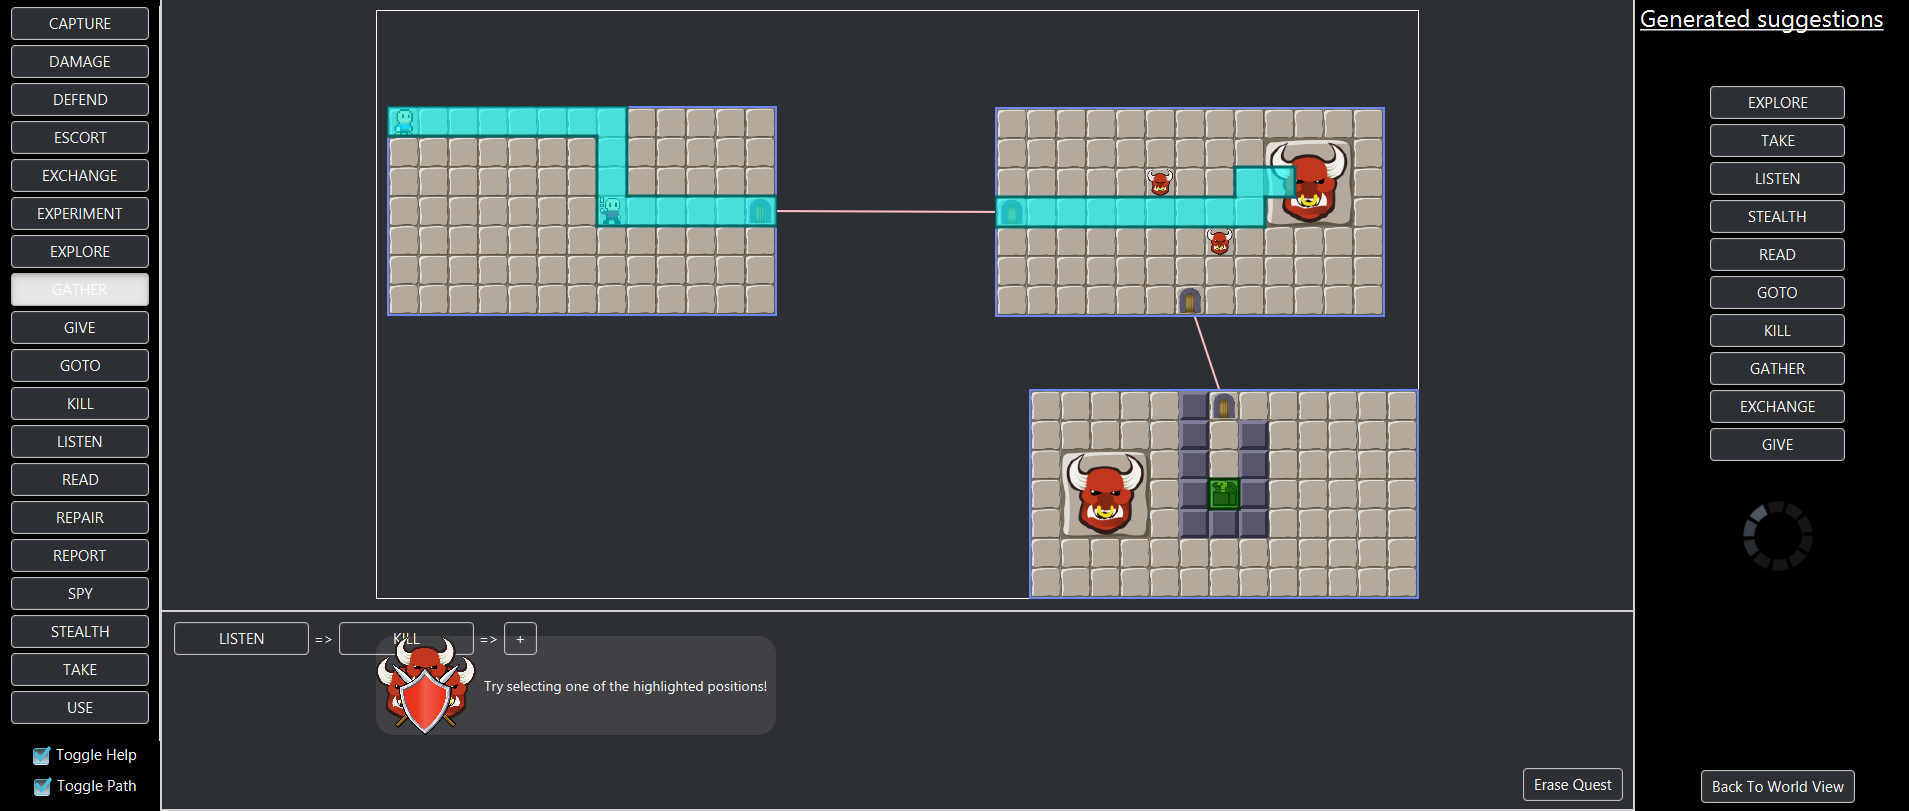
\includegraphics[width=\textwidth]{figures/main-help.png} %temp
%     \caption{The Story Designer screen in EDD.}
%     \label{fig:story-screen}
% \end{figure*}

% \begin{itemize}
% \item Brief intro to the tool's purpose. %done
% \item Subsection about story structures with TVtropes, node types, connection types, examples %done
% \item Subsection with EDD's story structure creation view. %done
% \item Subsection with representing and evolving with Graph Grammars in EDD 
% \end{itemize}

% \begin{table*}[ht]
% \centering
\caption{General consensus on EDD's features} \label{p1tab:consensus}
\resizebox{0.8\textwidth}{!}{
\begin{tabularx}{\textwidth}{|p{0.2\textwidth}|p{0.99\textwidth}|}
\cline{1-2}

Description & Participants’ Consensus \\\cline{1-2}
World Grid  of the dungeon                   & Its purpose of establishing an illusion of a fully realized dungeon is somewhat achieved. However, limitations exist with how it defines feasibility, a dungeon’s starting point, and the entrances, which disrupts the designers’ decisions.                                                                                                                                                                                   \\\cline{1-2}
World View                                  & The world view’s usefulness for the most part could not be established, other than for the purpose of going to the suggestions view (which was already seldom during the user study) and having a closer look at the entire dungeon without any distractions. Some participants preferred features to be already in the room view’s minimap, and some wanted to see more specific functionalities within the world view itself. \\\cline{1-2}

Enabling and  \newline disabling rooms                & As the user study restricted participants to create 3x3 dungeons, this feature for the most part has been neglected. This is also in part because of its accessibility only being in the world view, which proved to be an inefficient view in general. However, its use for bigger dungeon sizes later on was appreciated, especially for more intricate design purposes.                                                      \\\cline{1-2}
Suggestions View                            & Similarly to enabling and disabling rooms, it was quite difficult to encourage the use of this functionality due to the world view’s inefficient usability. However, this could also be due to the dungeon’s small size, as some participants expressed high interest in using more suggestions with larger dungeon sizes.                                                                                                      \\\cline{1-2}
Minimap  \newline  navigation                      & The minimap proved to be a strong tool not only for navigation purposes, but also for supporting design decisions and choices. The directional buttons were rarely used, but their room previews were helpful in emphasizing the current room’s connection to adjacent rooms without looking at the minimap. On the other hand, this lowered the usability of the world view.                                                   \\\cline{1-2}
Parameters                                       & The parameters were, in general, lacking. They served to be important in decision-making when choosing a suggested map in room view, but there were still doubts on their accuracy and sufficiency when providing information about the generated suggestions.                                                                                                                                                                       \\\cline{1-2}
Generated maps for  \newline  suggestions in room view & Suggestions in the room view proved to be very helpful in supporting the whole design process as they primarily acted as inspirations for the users. The most prominent comment among the users is the preference of having more control on how suggestions should be generated depending on different types of parameters.                                                                                                     \\\cline{1-2}
Design \newline  patterns& The patterns’ visualization was, in general, lacking and not self-explanatory. Some participants have expressed interest in using patterns as a parameter in the generation of suggestions.                                                                                                                                                                                                                                     \\\cline{1-2}
Dark theme                                  & EDD’s dark theme for the user interface received a positive response as it makes working with the program easier.
	\\ \cline{1-2}
\end{tabularx}
}
\end{table*}

% \begin{table}
% \begin{center}
% {\caption{Best performing setups based on their internal validation and visualization of clustered data points.}\label{table:setups}}
% \resizebox{\textwidth}{!}{
% \begin{tabular}{ccccccc}
% \hline
% \rule{0pt}{12pt}
% Algorithm&Data&K&$\Diamond$&$\Box$&$\bigtriangleup$ 
% \\ 
% \hline
% \\[-6pt]
% K-Means & Tiles-PCA & 9 & 0.43 & 0.73 & 9438.233 \\ 
% K-Means & Tiles-PCA & 12 & 0.41 & 0.77 & 9436.928 \\
% K-Means & Dimensions-PCA & 12 & 0.43 & 0.73 & 7738.343 \\
% Agglomerative single & Combined-PCA & 6 & 0.51 & 0.43  & 38.833 \\ 
% Agglomerative avg. & Dimensions-PCA & 6 & 0.44 & 0.67 & 3463.567 \\ 
% \hline
% \\[-6pt]
% \multicolumn{6}{l}{$\Diamond$ Silhouette Score\ \
% $\Box$ Davies Bouldin Index\ \
% $\bigtriangleup$ Calinski-Harabasz Index}
% \end{tabular}
% }\end{center}
% \end{table}

% \begin{itemize}
%     \item Brief intro to the tool's purpose.
%     \item Subsection about TropeTwist briefly explaining how tropes are used and the trope patterns. story structures with TVtropes, node types, connection types, examples done \checkmark
%     \item Subsection with EDD's story structure creation view, and workflow. \checkmark
%     \item Add info on the development from questgram with specific NPCs and the questview changed (although, that last part is not relevant). Also add the info on how to actually use this system.
%     \item Brief subsection with how graph gramamrs work and how we represent these graphs for the EA. Not super in detail because all of that is from tropetwist. 
%     \item The things that are extended in this version is the amount of dimensions, and how the elites are shown! (besides actually showing all of this!)
%     \item Dimensions should be addressed in the final subsection. 
%     \item How elites are shown and all of that goes to the workflow subsection.
% \end{itemize}


%\begin{figure*}[t!]
%    \centering
%    \includegraphics[width=\textwidth]{figures/current_GUI.png}
%    \caption{The Story Designer screen in EDD.}
%    \label{fig:story-screen}
%\end{figure*}
 
% \begin{table*}[ht]
% \centering
\caption{General consensus on EDD's features} \label{p1tab:consensus}
\resizebox{0.8\textwidth}{!}{
\begin{tabularx}{\textwidth}{|p{0.2\textwidth}|p{0.99\textwidth}|}
\cline{1-2}

Description & Participants’ Consensus \\\cline{1-2}
World Grid  of the dungeon                   & Its purpose of establishing an illusion of a fully realized dungeon is somewhat achieved. However, limitations exist with how it defines feasibility, a dungeon’s starting point, and the entrances, which disrupts the designers’ decisions.                                                                                                                                                                                   \\\cline{1-2}
World View                                  & The world view’s usefulness for the most part could not be established, other than for the purpose of going to the suggestions view (which was already seldom during the user study) and having a closer look at the entire dungeon without any distractions. Some participants preferred features to be already in the room view’s minimap, and some wanted to see more specific functionalities within the world view itself. \\\cline{1-2}

Enabling and  \newline disabling rooms                & As the user study restricted participants to create 3x3 dungeons, this feature for the most part has been neglected. This is also in part because of its accessibility only being in the world view, which proved to be an inefficient view in general. However, its use for bigger dungeon sizes later on was appreciated, especially for more intricate design purposes.                                                      \\\cline{1-2}
Suggestions View                            & Similarly to enabling and disabling rooms, it was quite difficult to encourage the use of this functionality due to the world view’s inefficient usability. However, this could also be due to the dungeon’s small size, as some participants expressed high interest in using more suggestions with larger dungeon sizes.                                                                                                      \\\cline{1-2}
Minimap  \newline  navigation                      & The minimap proved to be a strong tool not only for navigation purposes, but also for supporting design decisions and choices. The directional buttons were rarely used, but their room previews were helpful in emphasizing the current room’s connection to adjacent rooms without looking at the minimap. On the other hand, this lowered the usability of the world view.                                                   \\\cline{1-2}
Parameters                                       & The parameters were, in general, lacking. They served to be important in decision-making when choosing a suggested map in room view, but there were still doubts on their accuracy and sufficiency when providing information about the generated suggestions.                                                                                                                                                                       \\\cline{1-2}
Generated maps for  \newline  suggestions in room view & Suggestions in the room view proved to be very helpful in supporting the whole design process as they primarily acted as inspirations for the users. The most prominent comment among the users is the preference of having more control on how suggestions should be generated depending on different types of parameters.                                                                                                     \\\cline{1-2}
Design \newline  patterns& The patterns’ visualization was, in general, lacking and not self-explanatory. Some participants have expressed interest in using patterns as a parameter in the generation of suggestions.                                                                                                                                                                                                                                     \\\cline{1-2}
Dark theme                                  & EDD’s dark theme for the user interface received a positive response as it makes working with the program easier.
	\\ \cline{1-2}
\end{tabularx}
}
\end{table*}

% \begin{table}
% \begin{center}
% {\caption{Best performing setups based on their internal validation and visualization of clustered data points.}\label{table:setups}}
% \resizebox{\textwidth}{!}{
% \begin{tabular}{ccccccc}
% \hline
% \rule{0pt}{12pt}
% Algorithm&Data&K&$\Diamond$&$\Box$&$\bigtriangleup$ 
% \\ 
% \hline
% \\[-6pt]
% K-Means & Tiles-PCA & 9 & 0.43 & 0.73 & 9438.233 \\ 
% K-Means & Tiles-PCA & 12 & 0.41 & 0.77 & 9436.928 \\
% K-Means & Dimensions-PCA & 12 & 0.43 & 0.73 & 7738.343 \\
% Agglomerative single & Combined-PCA & 6 & 0.51 & 0.43  & 38.833 \\ 
% Agglomerative avg. & Dimensions-PCA & 6 & 0.44 & 0.67 & 3463.567 \\ 
% \hline
% \\[-6pt]
% \multicolumn{6}{l}{$\Diamond$ Silhouette Score\ \
% $\Box$ Davies Bouldin Index\ \
% $\bigtriangleup$ Calinski-Harabasz Index}
% \end{tabular}
% }\end{center}
% \end{table}

Story Designer is a new system integrated in EDD, which presents a visual interface for mixed-initiative narrative structure generation. It makes extensive use of the TropeTwist system as foundation to build narrative graphs and assess them by identifying trope patterns. The user manually designs a story structure by adding and interconnecting nodes in a graph, which seeds an evolutionary algorithm (EA) that generates story structure suggestions that can be incorporated into the user's design. This continuous co-creative design process implements the Interactive Constrained MAP-Elites (IC MAP-Elites) approach presented in~\cite{p11alvarez_empowering_2019}, providing quality-diverse suggestions across several feature-dimensions.

Story Designer is interconnected with the level design facet in EDD. This means that the narrative graphs that can be developed and that can be generated and suggested are constrained by the content that exists in the levels. For instance, if the designer adds two NPCs besides the Hero, then the system could at most, use three character nodes to represent them, or if the designer adds a boss enemy and a quest item, this would mean that the boss enemy could be represented as one of the villain nodes (e.g., Enemy, Big Bad, or Dragon) and the quest item as a possible Plot Device.

\subsubsection{TropeTwist}

TropeTwist~\cite{p11alvarez_tropetwist_2022} is a system that uses tropes~\cite{p11lewis_governing_2018,garcia-sanchez_simpsons_2021,richmond_tv_2004,harris_periodic_2016}, narrative conventions easily recognizable by the audience, as patterns that combine to compose narrative structures. These structures define generic aspects of a story, leading to the identification of events, roles, and other relevant narrative elements arranged as nodes in an interconnected narrative graph. By having all this elements in a graph, entire narratives are encoded using graph grammars, to then procedurally generate novel narrative variations by means of a MAP-Elites algorithm that considers several narrative evaluation metrics, such as interestingness, coherence, and cohesion. 

Nodes in a narrative graph represent tropes. Interconnected tropes create other composite tropes and patterns, that can be identified as subgraphs of a complete narrative graph. These patterns can be \textbf{micro-patterns} encapsulating a single trope node, \textbf{meso-patterns}, often composed by more than one micro-pattern with a specific meaning, and \textbf{auxiliary patterns}, identifying structural gaps in the graph. For a detailed definition of all tropes and patterns, please refer to~\cite{p11alvarez_tropetwist_2022}. Here we present a comprehensive summary:

\begin{itemize}
    \item Micro-patterns are the fundamental narrative unit in the system, encapsulating tropes in building blocks to create complex narrative structures. These are classified into structure patterns (SP), that articulate the story elements (i.e. Conflict), character patterns (CP) (i.e. heroes and villains), and plot device patterns (PDP), that move the story forwards towards a particular goal (i.e. the MacGuffin).
    \item Meso-patterns may emerge from the combination of micro-patterns and other meso-patterns, denoting spatial, semantic, and usability relationship within the narrative graph.
    \begin{enumerate}
        \item The \emph{Conflict Pattern (ConfP)} ties a conflict node to two other nodes representing both parties in a conflict (i.e. HERO $\rightarrow$ CONFLICT $\rightarrow$ EMP, a hero is in conflict with the Empire).
        \item The \emph{Derivative Pattern (DerP)} defines relations of entailment between other nodes, called derivatives. These derivatives acquire a local and temporal order, and a causal relationship. I.e the former conflict connected to EMP $\diamondsuit$--- DRA $\diamondsuit$--- NEO, means that the hero engages the Empire, which entails both a conflict with the Dragon (\emph{DRA}) and the appearance of the Chosen One (\emph{NEO}).
        \item The \emph{Reveal Pattern (RevP)} connects two independent CPs as one, meaning that character A was, in fact, always character B, and vice-versa. This pattern turns all existing conflicts between them into \emph{fake} conflicts.
        \item The \emph{Active Plot Device Pattern (APD)} triggers a PDP and integrates it in the the narrative, since PDP are passively described and lack any start condition.
        \item \emph{Plot Points (PP)} are key discrete narrative events. The derivatives within a \textit{DerP}, the source of a reveal pattern, as well as active plot devices are considered plot points.
        \item A \emph{Plot Twist (PT)} identifies those plot points that could change the natural flow of the narrative. I.e. in EMP $\diamondsuit$--- DRA $\diamondsuit$--- NEO, NEO is identified as a plot twist since its nature (heroic) is opposed to that of the first node EMP (villainous), which alters the natural order of the connecting derivative pattern.
    \end{enumerate}
    \item Auxiliary patterns spot and encapsulate those areas in the graph that don't contain meaningful narrative information. \textit{Nothing} highlights nodes that are not identified or part of any meso-pattern; whereas \textit{Broken Link} marks outgoing connections from any node that do not lead to any pattern.
\end{itemize}



\subsubsection{Workflow}


Story Designer is integrated in EDD as a separate view (Figure \ref{fig:story-screen}) that can be accessed anytime from the dungeon editor. The use starts with a minimal sample narrative graph HERO $\rightarrow$ CONFLICT $\rightarrow$ ENEMY in the manual edition pane (center). This graph can be extended by adding nodes from the node context menu that pops up with a right-click on an empty space. Node are arranged by type for the sake of clarity, and an option to automatically re-arrange the graph is shown at the end of the menu. Right-clicking on an existing node border will pop up the edge context menu, that allows the user to create a new connection or to delete the selected node. Existing connections are deleted by left-clicking on them.

In a way similar to EDD's room editor \cite{p11alvarez_empowering_2019}, as the user edits the narrative graph manually, this graph is fed into the underlying evolutionary algorithm that procedurally generates on the fly alternative narrative graphs in the suggestions pane (right). The top-right corner shows the feature-dimension matrix, whose cells are colored depending on the fitness of the fittest elite contained in it, ranging from dark red (no elite yet), to dark green (optimal fitness). The elite in the selected cell of the matrix is displayed in the bottom-right corner. Hovering the mouse above a cell displays its elite's graph above the selected one, which allows the user to compare several graphs at a glance.    

%\subsubsection{Building stories with tropes}

%In storytelling, a trope \cite{p11garcia-sanchez_simpsons_2021} is a convention or figure of speech that is assumed by the storyteller to be easily recognizable by the audience. TV tropes is an online wiki and repository that compiles, curates, and describes several thousands of tropes in many sorts of media, such as television, films, literature, and games \cite{p11richmond_tv_2004}. As exemplified by \cite{p11harris_periodic_2016}, tropes can be interconnected in graph-like structures, called story molecules, to succinctly depict the story behind a narrative in any common media.

%Story Designer elaborates on the concept of story molecule as a means to represent stories using graph-like structures of interconnected tropes, called narrative graphs. Table \ref{tab:tropes} shows all the tropes that can be added as nodes to a narrative graph, represented by their symbol. Nodes are depicted with shapes specific to their trope type: heroes (rectangle), conflicts (diamond), enemies (hexagon), and plot devices (circle).

%Nodes in a narrative graph are necessarily interconnected by either unidirectional or bidirectional edges (with one or both arrow heads), or by entailment edges (with a single diamond head). Given nodes A and B, A $\diamondsuit$--- B reads as "A entails B", whereas A $\rightarrow$ B denotes a relationship from A to B, and B $\rightarrow$ A the opposite. A $\leftrightarrow$ B denotes a reflexive relationship between A and B. As an example, HERO $\rightarrow$ CONFLICT $\rightarrow$ EMP denotes a hero who is in conflict against an empire-type enemy, whereas HERO $\leftrightarrow$ CONFLICT denotes a hero who is in conflict with herself. EMP $\diamondsuit$--- DRA $\diamondsuit$--- NEO, denotes an empire that entails a dragon enemy that, once beaten, will lead to the appearance of a chosen one hero.



%\subsubsection{Trope Patterns}

%\begin{itemize}
%    \item This has to be reduced considerably to simply introduce the terms but link the reader to the TropeTwist paper! (Add it to Arxiv)!
%    \item Micro: Micro-patterns are the fundamental unit in the system which aims at categorizing different sets of the individuals patterns that are shown in table~\ref{tab:tropes}. Micro-patterns are the basic building block which when connected together allows the detection of meso-patterns.  (AND WRITE THEM)
%    \item Meso: If micro-patterns are the fundamental units to construct narratives in StoryDesigner, then Meso-patterns are the features~\cite{p11dahlskog_multi-level_2014} that emerge in the narrative from dynamically combining micro-patterns and in some occasions these with meso-patterns. Meso-patterns are composite patterns, always composed by more than one pattern denoting some spatial, semantic, and usability relationship within the narrative graph. Micro-, meso-, and macro-patterns have been used to generalize the generation of content and reduce the burden and complexity of generators mainly in regards to evaluation and encoding of the content, as well as a tool to compare generated or human-authored content. For StoryDesigner and the creation of narratives, we have identified a subset of Tropes (extracted from TVTropes) that require (or work as) the combination between more fundamental units. For instance, the reveal pattern relates to the "Good all along" or "evil all along" tropes from TVTropes. (AND WRITE THEM)
%    \item AUXILIARY: Denotes problems in the graph, and sub-optimal and impractical nodes and connections within a graph. (AND WRITE THEM)
%\end{itemize}

%\subsubsection{TropeTwist}

%------------------------------

% \subsubsection{Trope Patterns}

%\subsubsection{Tropes as Patterns}

% Given the nature of tropes as recognizable parts of stories
% The system analyzes the possible tropes to us

% All patterns calculate their quality, which is then used in different ways to estimate the quality and fitness of narrative structures.

% In most of the patterns that will be described we calculate and use two general qualities, which are indicated when used. The first quality is the $generic_{qual}(pattern)$, which uses the occurrence of the specific pattern within the edited graph by the user and is calculated as:

% \begin{equation}
%     quantity_{qual}(pattern) = pattern \sim \mathcal{N}(\mu,\,\sigma^{2})\,.
% \end{equation}

% where...

% The second general quality used to calculate the quality of the tropes is the $quantity_{qual}(pattern, trope)$, which uses the occurrence of a trope of a specific pattern class within the tested graph, and is calculated as:

% \begin{equation}
%     repetition_{qual}(pattern, trope) = \dfrac{\sum_{i=0}^{\left | patterns \right |}}{\left | pattern \right |}
% \end{equation}

% where $p$ is defined as the specific patterns within  $p = pattern \in AllPatterns$,

% \paragraph{Micro-Patterns}

% Micro-patterns are the fundamental unit in the system which aims at categorizing different sets of the individuals patterns that are shown in table~\ref{tab:tropes}. Micro-patterns are the basic building block which when connected together allows the detection of meso-patterns. 

% \paragraph{Structure Pattern}

% An structure pattern (SP) is any type of trope that would give some structural definition to a narrative, whether this being a conflict, specific act, or a part in a dramatic arc (e.g., climax). In Story Designer, the only type of structure trope is the \textsc{conflict} (C) trope, which represents the most basic structural interaction. The quality $SP_{qual}$ is calculated as the normalized linear combination of:

% \begin{equation}
%     SP_{qual} = generic_{qual}(SP) + involvement_{qual}(SP)
% \end{equation}

% \paragraph{Hero Pattern}

% Hero patterns (HP) are good characters within the narrative that could potentially be the main hero of the narrative or complementary roles. In Story Designer, \textsc{HERO}, \textsc{5MA}, \textsc{NEO}, \textsc{SH} are classified as HP. HPs are commonly used as source or targets (or both) of other patterns and in a few special occasions to denote a relation to another character. The quality $HP_{qual}$ is calculated as the normalized linear combination of:

% \begin{equation}
%     HP_{qual} = generic_{qual}(HP) + quantity_{qual}(HP) + involvement_{qual}(HP)
% \end{equation}

% \paragraph{Villain Pattern}

% Villain patterns (VP) are by nature, evil characters within the narrative that could be the antagonist of the narrative, an elite enemy, or a faction\footnote{Having more than one villain in the narrative structure effectively establishes the bosses as \textit{Disc-One Final Boss} \url{https://tvtropes.org/pmwiki/pmwiki.php/Main/DiscOneFinalBoss}}. In Story Designer, \textsc{ENEMY}, \textsc{EMP}, \textsc{BAD}, \textsc{DRA} are classified as VP. As the opposite of the HPs, VPs properties and usages are mirrored. The quality $VP_{qual}$ is calculated as the normalized linear combination of:

% \begin{equation}
%     VP_{qual} = generic_{qual}(VP) + quantity_{qual}(VP) + involvement_{qual}(VP)
% \end{equation}

% \paragraph{Plot Device Pattern}

% Plot device patterns (PDP), are described as the element within the narrative moves it forward, in the shape of a goal, object, or dramatic element to be used or encountered by any of the characters. The quality $PDP_{qual}$ is calculated as the normalized linear combination of:

% \begin{equation}
%     PDP_{qual} = generic_{qual}(PD) + quantity_{qual}(PDP)
% \end{equation}


% \paragraph{Meso-Patterns}

% If micro-patterns are the fundamental units to construct narratives in StoryDesigner, then Meso-patterns are the features~\cite{p11dahlskog2014-multimultilevel} that emerge in the narrative from dynamically combining micro-patterns and in some occasions these with meso-patterns. Meso-patterns are composite patterns, always composed by more than one pattern denoting some spatial, semantic, and usability relationship within the narrative graph. Micro-, meso-, and macro-patterns have been used to generalize the generation of content and reduce the burden and complexity of generators mainly in regards to evaluation and encoding of the content, as well as a tool to compare generated or human-authored content. For StoryDesigner and the creation of narratives, we have identified a subset of Tropes (extracted from TVTropes) that require (or work as) the combination between more fundamental units. For instance, the reveal pattern relates to the "Good all along" or "evil all along" tropes from TVTropes

% %In StoryDesigner and for the creation of narratives, we have identif
% %Meso-patterns are features 
% %Meso-patterns are composite patterns, which combine or effectively utilizes several micro-patterns or other meso-patterns to produce 
% %Meso-patterns are the combination
% % Micro-patterns are the fundamental unit in the system which aims at categorizing different sets of the individuals patterns that are shown in table~\ref{tab:tropes}. Micro-patterns are the basic building block which when connected together allows the detection of meso-patterns. 

% \paragraph{Conflict Pattern} Relates to the conflict between two character micro-patterns (HPs or VPs). A conflict $C$ is formally defined as $\langle s, C, t \rangle$ where s and t are a character micro-pattern (i.e., either hero pattern or villain pattern). $C$ denotes the general conflict trope, which can be simple conflict (c), conflict against nature (cona), or conflict against society (coso). A conflict meso-pattern do not necessarily describe a conflict between two different characters, as conflicts can be self-conflicts expressed as a bi-directional connection between the character trope and conflict trope. This effectively makes $s$ and $t$ the same. 

% Moreover, a conflict pattern is either~\textsc{explicit} or~\textsc{implicit} as depicted in figure~\ref{fig:conflict_pattern_a} and~\ref{fig:conflict_pattern_b}. \textsc{Explicit Conflicts} are the ones that are explicitly encoded in the graph and directed from a source $s$ to a target $t$ passing through the conflict trope $C$. On the other hand, \textsc{Implicit Conflicts} relates to the conflicts from a target $t$ (or derivatives) to a source $s$ (or derivatives) that are not encoded in the graph. For instance, if a hero has an explicit conflict with an enemy, but the enemy does not, that produces an implicit conflict from enemy to hero. Conflicts are the main way of representing some type of structure and groups within StoryDesigner, and as seen before in the micro-pattern definition, they play a crucial role in their quality. The quality $ConfP_{qual}$ is calculated as the normalized linear combination of:

% \begin{equation}
%     ConfP_{qual} = generic_{qual}(ConfP) + quantity_{qual}(ConfP) + involvement_{qual}(ConfP)
% \end{equation}

% % and must be opposite to each other (e.g., if $s$ is a hero pattern, then $t$ must be a villain pattern.
% % \paragraph{Implicit Conflict Pattern}
% \paragraph{Composite Conflict Pattern} very simple, works as a grouper for a set of conflict patterns united by the same \textit{structure pattern}. This means, that if the same structure pattern is responsible (or is used) to establish $n$ amount of conflicts, then there will be $n$ amount of conflict patterns, and they will all be encapsulated within one composite conflict pattern. This is beneficial when we need to check and evaluate properties of the conflicts, such as the amount of conflicts associated to one single structure pattern (burdening) or the amount of self-conflicts. Due to this nature, CCP do not calculate a quality per se, rather their quality is cumulative from all the $ConfP$ they contain normalized by the amount of $ConfP$. 
% %there will be one CCP 

% \paragraph{Derivative Pattern} Derivatives defines a relationship between tropes connected by "entails" connections ($\diamondsuit$---). Derivatives start from a root micro-pattern and continue until no more "entail" connections are encounter, effectively establishing a hierarchy from the root to the derivatives. By design, the patterns within a derivative pattern have a local and temporal order, and a causal relationship. For instance, in the example given at the start of this section (EMP $\diamondsuit$--- DRA $\diamondsuit$--- NEO); having a conflict or engaging with the \emph{EMP}, entails both the conflict with \emph{DRA} and the appearance of \emph{NEO}. In this context, this means that only by "beating", "winning against", or any other way of overcoming the \emph{DRA} we will make \textit{narrative space} for \emph{NEO} to appear - as a new hero or the evolution of another. The \textit{narrative space} is crucial as it helps building up situations and plot points, and create meaningful interactions. The quality of a derivative pattern $Derp_{qual}$ is calculated based on its quantity on the target narrative graph, the balance of derivatives within this pattern using a gaussian bell centered on the avg. in the tested narrative graph ($\theta$), and the diversity of the derivatives.

% \begin{equation}
%     Derp_{qual} = generic_{qual}(Derp) + 
%     \theta + 
%     \frac{\sum_{i=0}^{|Derp_{der}|}i_{base}}{|Derp_{der}|}
% \end{equation}

% % , and have, by design, a local temporal order and causal 

% \paragraph{Reveal Pattern} A reveal connects two independent characters as one, meaning that character A was in fact always character B, and vice-versa. This pattern serves for creating confusion and surprise within a narrative structure, as for instance, a villain could have been in fact "Good All Along"\footnote{https://tvtropes.org/pmwiki/pmwiki.php/Main/GoodAllAlong}. In practice, a reveal pattern is identified as a villain or hero connected with a uni-directional connection ($\rightarrow$) to a hero or villain, respectively. As a consequence, all existing conflicts between factions would become \emph{fake}. $rev_{qual}$ is calculated based on its quantity on the target narrative graph, the amount of total reveals in the tested narrative graph in relation to characters, and the amount of generated fake conflicts given this specific reveal.

% \begin{equation}
%     rev_{qual} = generic_{qual}(rev) + repetition_{qual}(rev) + \Bigg( 1.0 - \frac{\sum_{i=0}^{|conf|}    \begin{cases}
%         1,& \text{if } rev \in x_{i}\\
%         0,              & \text{otherwise}
%     \end{cases}}{|ng_{conf}|} \Bigg)
% \end{equation}

% % the balance of derivatives within this pattern using a gaussian bell centered on the avg. in the tested narrative graph ($\theta$), and the diversity of the derivatives. 

% % Reveal patterns connect and relate a character with an opposing, as both are the same but in different factions.

% \paragraph{Active Plot Device Pattern} Plot device patterns by themselves only describe a goal or target to be achieved within a narrative. However, they do not operationalize and integrate those within the narrative. Once an PDP is in use by connecting to another micro-pattern and having other micro-patterns connected to it, then they do key contributions to the narrative. Almost all narrative make use of a plot device to move forward the story; thus, in Story Designer PDPs get utilize quickly as well. In practice, an \textit{APD} is identified as PDPs that contains at least any one connection to them, and optionally, one single output connection. These limitation is added to limit the effect of a PDP wihthin a narrative. The $APD_{qual}$ is measured based on the amount of APDs within the target graph, and the APD's usability, calculated based on the amount of incoming connections and output normalized using a gaussian bell centered on the half size of the tester narrative graph defined as $\theta$. Usability is calculated like this to penalize APDs that do not use as many connections as possible but neither be the only APD in place.

% \begin{equation}
%     APD_{qual} = generic_{qual}(APD) + \theta
% \end{equation}


% \paragraph{Plot Elements} 

% Plot elements are treated as composite patterns and meso-patterns, but rather than pointing some underlying trope such as \emph{reveal}, they describe key elements within the current narrative structure. Plot elements can then be used to assess semantically the narrative graph and to inform other systems about main events within the structure.

% % They are technically composite patterns as the meso-patterns, but are linked to plot information and description.

% \paragraph{Plot Points} Plot points are key events happening within the narrative graph, identified as discrete moments given some pattern. At the moment, we consider as plot points, the derivatives within a \textit{Derivative pattern}, the reveal pattern's source, and the plot devices that are \textit{Activate plot Device}. Quality $PP_{qual}$ is measured based on the amount of PPs within the target narrative graph, and the amount of PPs within the tested narrative graph, in relation to the nodes within it.

% \begin{equation}
%     PP_{qual} = generic_{qual}(PP) + quantity_{qual}(PP)
% \end{equation}

% \paragraph{Plot Twist} Plot twists take advantage of plot points to identify those that could have a bigger impact, surprise a player, or change drastically the narrative. In practice, \emph{PTs} consider the source of \textit{RevP}, derivatives from \textit{DerP} that are a different micro-pattern than the root, and \textit{APDs} that are connected to other \textit{APDs}. For instance, reusing the same example of EMP $\diamondsuit$--- DRA $\diamondsuit$--- NEO, given that NEO is a different micro-pattern than root EMP, this will be identified as a \textit{Plot Twist} as it alters the "natural" order in the derivative. PTs quality ($PT_{qual}$) is based on the amount of PTs within a target narrative graph, the PT's degree of involvement in the narrative, and the balance of PTs in function of the PPs in the tested narrative graph. When a PT is related to a \textit{RevP}, involvement is calculated as how much the structure changes based on that (i.e., how many fake conflicts are created). When it is related to \textit{DerP}, involvement is calcualted as how different the pattern is and its order within the derivatives. Finally, when it is related to \textit{APD}, involvement is based on how usable the \textit{APD} is within the narrative based on incoming and outgoing connections.

% \begin{equation}
%     PT_{qual} = generic_{qual}(PT) + involvement_{qual}(PT, assoc_{pat}) + \frac{|ng_{pt}|}{|ng_{pp}|}
% \end{equation}

% \paragraph{Auxiliary Patterns}

% Denotes problems in the graph, and sub-optimal and impractical nodes and connections within a graph.

% \paragraph{Nothing} Nodes that are not assigned or identified within any of the meso-patterns, are categorized as \textit{Nothing} within Story Designer. This means that their contribution to the overall narrative is none-existent; thus, pointing towards "degenerated" narratives. 
% \paragraph{Broken Link} A node might be useful within a narrative but not all of its connections. Therefore, unused connections within a graph are assigned a \textit{Broken Link} pattern to identify those that do not contribute to a coherent and interesting narrative structure.

% \paragraph{Micro-Patterns}

% \paragraph{Structure Pattern}
% \paragraph{Hero Pattern}
% \paragraph{Villain Pattern}
% \paragraph{Plot Device Pattern}

% \paragraph{Meso-Patterns}

% \paragraph{Conflict Pattern} Relates to the conflict between two character micro-patterns. A conflict $C$ is formally defined as $\langle s, C, t \rangle$ where s and t are a character micro-pattern (i.e., either hero pattern or villain pattern). $C$ denotes the general conflict trope, which can be simple conflict (c), conflict against nature (cona), or conflict against society (coso). A conflict meso-pattern do not necessarily describe a conflict between two different characters, as conflicts can be self-conflicts expressed as a bi-directional connection between the character trope and conflict trope. This effectively makes $s$ and $t$ the same. 

% Moreover, a conflict pattern is either~\textsc{explicit} or~\textsc{implicit}. 

% % and must be opposite to each other (e.g., if $s$ is a hero pattern, then $t$ must be a villain pattern.
% % \paragraph{Implicit Conflict Pattern}
% \paragraph{Composite Conflict Pattern}
% \paragraph{Derivative Pattern}
% \paragraph{Reveal Pattern}


% \paragraph{Plot Elements}

% \paragraph{Plot Points}
% \paragraph{Active Plot Device Pattern}
% \paragraph{Plot Twist}

% \paragraph{Auxiliary Patterns}

% \paragraph{Nothing}
% \paragraph{Broken Link}




\subsubsection{Evolving narrative structures with Graph Grammars}

The underlying evolutionary algorithm in Story Designer is an adapted version of IC MAP-Elites~\cite{p11alvarez_interactive_2020} to evolve grammars. In Story Designer, an individual's phenotype is a narrative graph, and its encoding genotype is a graph grammar. A graph grammar is a context-free grammar whose productions add, remove, and modify nodes and edges to a graph. 

An individual's genotype is the production rules of the grammar, which are deterministic i.e., a production rule (or pattern) only matches one production. Given that the graph grammar does not need to be applied sequentially until terminal nodes are reached, every individual does a random sampling of the rules in their genotype to produce \emph{recipes}. \emph{Recipes} simply describe the order of rules to be applied (sequentially) and the amount of times they will be applied. \emph{Recipes} do not have repetitions within them i.e., if rule 1 is added at step 2, subsequent addition would simply add to the amount of times that rule will be applied at step 2. The internal parts of the EA works exactly as in TropeTwist, but now it is extended to use all the capabilities of IC MAP-Elites, namely, the continuous adaptive evolution aspect~\cite{p11alvarez_tropetwist_2022,alvarez_interactive_2020}.

%\begin{table}[]
\caption{Level constraints used per Experiment. Constraints were chosen based on the maximum amount of elements needed to design the narrative structure in the system.}
\begin{tabular}{l|llll}
Constraining elements & Exp. 1 & Exp. 2 & Exp. 3 & Exp. 4 \\ \hline
Heroes                & 2            & 2            & 4            & 2            \\
Enemies               & 2            & 2            & 1            & 2            \\
Quest Items           & 2            & 3            & 1            & 2           
\end{tabular}
\label{tab:level-constraints}
\end{table}

%Graph grammars do not apply rules sequentially; instead, every individual does a random sampling of the rules in their genotype to produce \emph{recipes} to generate a narrative graph. \emph{Recipes} describe the rules' order and repetition. \emph{Recipes} do not have repetitions within them, i.e., if rule 1 is added at step 2, subsequent addition would simply add to the number of times that rule will be applied at step 2. 

%The EA worksThe EA works exactly as 


%Our implementation uses the tropes listed in Table \ref{tab:tropes} as nodes, and the three available connection types as edges. Figure~\ref{fig:gen2phen} shows a sample complete process from an individual's genotype (i.e., rules) to the phenotype (i.e., narrative graph).

%Figure XXX shows a sample individual's genotype (grammar) and phenotype (narrative graph).

% individual's genotype is the production rules of the grammar, which are deterministic i.e., a production rule (or pattern) only matches one production. Given that the graph grammar does not need to be applied sequentially until terminal nodes are reached, every individual does a random sampling of the rules in their genotype to produce \emph{recipes}. \emph{Recipes} simply describe the order of rules to be applied (sequentially) and the amount of times they will be applied. \emph{Recipes} do not have repetitions within them i.e., if rule 1 is added at step 2, subsequent addition would simply add to the amount of times that rule will be applied at step 2. Given that production rules can grow without limit and are always minimum 2, the amount of recipes can escalate quickly (e.g., if we have 5 rules, the permutations are calculated as $5!$, resulting in 120 possible recipes without counting the amount of times the rule can be applied). Therefore, we limit the system and all experiments to $10$ recipes regardless of the chromosome size.

%Maybe show first the fitness evaluation and then go and jump to the dimensions.

Moreover, thanks to continuous evolution, the EA constantly incorporates the most recent version of the user’s design to the population of individuals in the corresponding cell of the feature-dimension matrix. The designer can switch between dimensions at any given time, as well as changing their granularity. IC MAP-Elites manages two different populations within each cell: a feasible and an infeasible one. Individuals move across cells when their dimension values change, or between the feasible and infeasible population according to their fulfillment of the feasibility constraint. Narrative graphs are deemed infeasible if they are not fully connected (i.e., all nodes can be reached from an arbitrary starting point), if there exist a conflict pattern within the graph with more than one self-conflict, or if level design constraints are enabled, the narrative graph violates any level design constraint. Infeasible individuals are evaluated (equation~\ref{eq:inf_fitness} in a weighted sum ($w_{0}=0.5, w_{1}=0.25, w_{2}=0.25$) based on how close they are to being fully connected and to remove inadequate self-conflicts, while trying to maximize the graph's cohesion.

%\begin{equation}
%\label{eq:cohesion_fitness}
%f(cohesion) = w_{0} *  \frac{\#NOT_{pat} + \#BROL_{pat}}{|V(NG)| \times 2} + w_{1} *  \frac{\#NOT_{pat} + \#BROL_{pat}}{\#micro_{pat} \times 2} 
%\end{equation}

\begin{multline}
\label{eq:inf_fitness}
f(infeasible) = w_{0} \times f(cohesion) + w_{1} \times \frac{\#!reachable_{V(NG)}}{|V(NG)|} 
\\ + w_{2} \times  \frac{\#!valid_{NG(self_conf)}}{|V(NG)|}
\end{multline}

Generated narrative graphs that are deemed feasible, are evaluated on their coherence (equation~\ref{eq:coherence_fitness}), which is used to assess how correct, coherent, and in general, syntactically correct the narrative graphs are. Coherence aims at maximizing an equally weighted sum between cohesion and consistency (eq.~\ref{eq:consistency_fitness}). Cohesion refers to the link between elements that hold together to form some group, which in Story Designer means the minimization of auxiliary patterns (\textit{Nothing} and \textit{Broken Link}) within the narrative graph. Consistency means that the narrative graph should be regular and free of contradictions, aiming at maximizing the quality of micro-patterns and minimize contradictions created by meso-patterns (contradictions can affect the consistency fitness up to $w_{0}=0.3$). For a more detailed explanation of how the EA works internally and the different fitness functions, we refer to the TropeTwist paper~\cite{p11alvarez_tropetwist_2022}.

%.. Thus, we calculate $f(consistency)$ as the collective quality of micro-patterns (regarded as fundamental units that should be somewhat regular and useful) normalized by the micro-pattern count $|micropat|$, and the goodness of explicit and implicit conflicts based on the amount of fake conflicts that exist. In effect, with consistency we aim at minimizing contradictions created by meso-patterns that affect micro-patterns and improving the general quality of the four micro-patterns.

%A consistent NG should be regular and free of contradictions. Thus, we calculate $f(consistency)$  (eq.~\ref{eq:consistency_fitness}) as the collective quality of micro-patterns since they are the building blocks, and conflicts' goodness based on the number of fake conflicts. In effect, with consistency, we aim to maximize the quality of micro-patterns and minimize contradictions created by meso-patterns.

%With cohesion, we focus on minimizing the   calculated as a equally weighted sum that aims at maxizming

%- Cohesion: Linking between words to hold together the text (how related the tropes are??)
 %*       --> Probably we can use something like, if a pattern is "nothing" there are cohesion problems?

%Coherence is calculated as a weighted sum ($w_{0}=0.7, w_{1}=0.3$)


%In addition to the feature-dimensions, all individuals are evaluated according to the following fitness function:

%\begin{equation}
%\label{eq:consistency_fitness}
%f(consistency) = w_{0} \times \frac{\sum_{i=0}^{|ng_{micro}|} i_{qual}}{|ng_{micropat}|} +  \\ 
%w_{1} \times \frac{|ng_{fakeConfP}|}{|ng_{confP}|} 
%\end{equation}

\begin{equation}
\label{eq:consistency_fitness}
f_{consistency} = \frac{\sum_{i=0}^{len(ng_{micro})} i_{qual}}{len(ng_{micropat})} -  \\ 
w_{0} \times \frac{len(ng_{fakeConfP})}{len(ng_{confP})} 
\end{equation}

\begin{equation}
\label{eq:coherence_fitness}
f(coherence) = f(consistency) + (1.0 - f(cohesion))
\end{equation}

\subsubsection{Behavior Dimensions for Graph Grammars}

Dimensions in MAP-Elites are a key component for the search space to be delimited, and are identified as those aspects of the individuals that can be calculated in the behavioral space, and that are independent of the fitness calculation. In Story Designer, the designer is able to pick two dimensions at a time to facilitate visualization, and all dimensions, when needed, are limited using a threshold $\delta = 5$. TropeTwist implemented \textit{Interestingness} and \textit{Step} as behavior dimensions when using MAP-Elites to generate novel narrative graphs. \textit{Step} is calculated as the Levenshtein distance between two narrative graphs, taking into account the amount of nodes and connections and their type (eq. \ref{eq:StepDim}). \textit{Interestingness} make use of the APDs, Plot Points, and Plot Twists that are present in a narrative graph to assess an approximate semantic evaluation since those represent some type of variation in the graph (eq.~\ref{eq:interesting_fitness}). Given \textit{Interestingness} is a highly subjective measurement, we rely on those patterns since they calculate their quality based on the current narrative graph and the one being edited by the designer.

\begin{equation}
\label{eq:StepDim}
D_{step} =  \frac{lev_{a,b} (|a|, |b|)}{\theta}
\end{equation}

\begin{equation}
\label{eq:interesting_fitness}
D_{int} = w_{0} \times \frac{APD_{q}}{\#APD} + w_{1} \times \frac{\#PP_{q}}{\#PP} +  w_{2} \times \frac{PT_{q}}{\#PT}ng
\end{equation}

Furthermore, we have extended TropeTwist with five more dimensions relevant to the narrative structure design process, to give more choice to designers and experiment with other dimensions in the search space:


%Furthermore, This EA is wrapped by an IC MAP-Elites \cite{p11alvarez} that evaluates each phenotype (narrative graph) according to the a set of feature-dimensions that assess different aspects of the narrative graphs:

%Given that the patterns active plot devices, plot points, and plot twists can have a high impact in the narrative graph and depend on several other patterns and specific structures, we limit all of then with threshold $\delta = 5$.

\begin{figure*}[t]
    \centering
    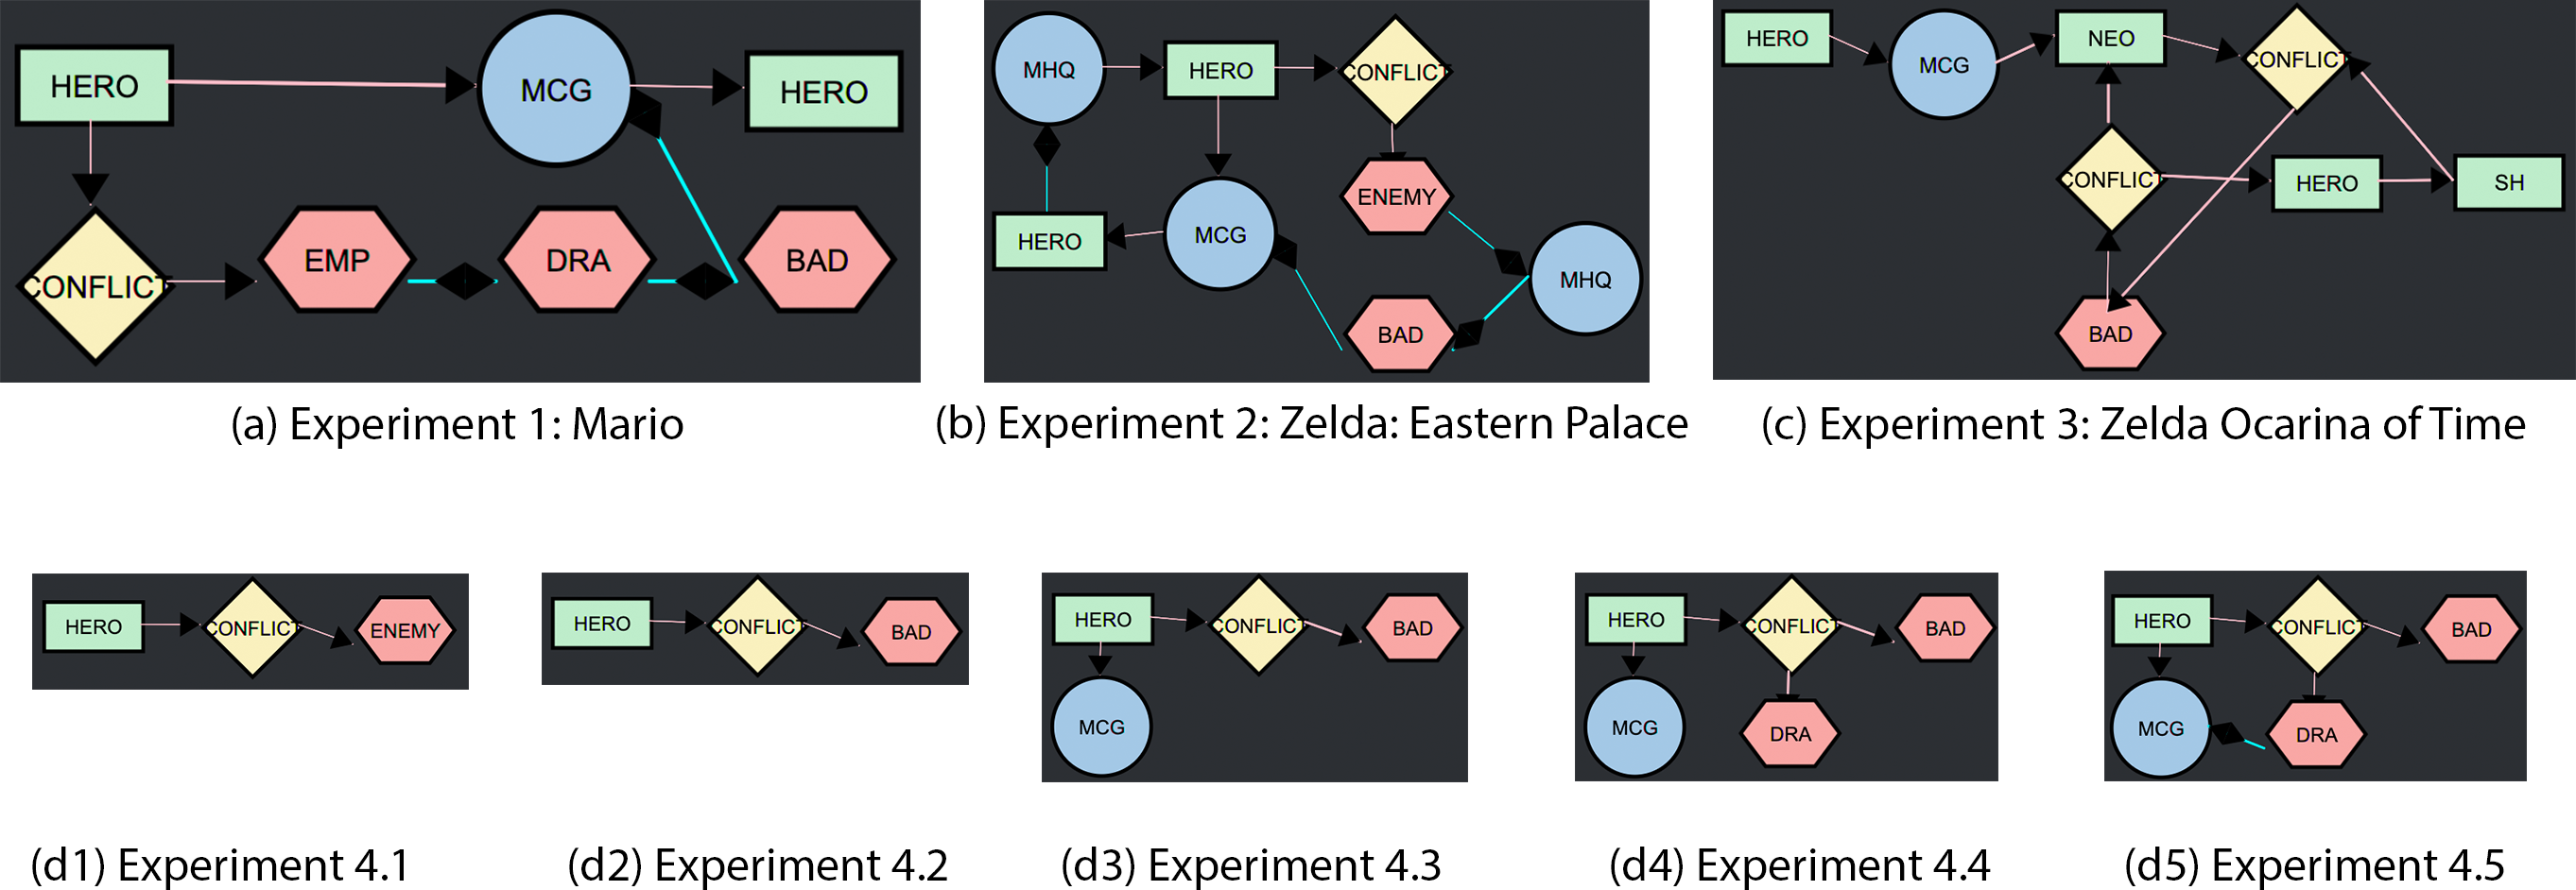
\includegraphics[width=\textwidth]{figures/example-experiments.png}
    \caption{Narrative graphs used for the experiments, constructed and designed in Story Designer. When experiment 4 is discussed, the narrative graph referred is Experiment 4.5 as that is the design's final step.}
    \label{fig:examples}
\end{figure*}

\textbf{Diversity (div).} Diversity measures the variety of [base] trope types within a narrative structure. Currently, there exist four base trope types, \textit{Hero} (h), \textit{Villain} (v), \textit{Structure} (s), \textit{Plot Devices} (pd). Diversity takes into account the tropes that also extend these base tropes. Thus, $D_{div}$ collects all tropes within a graph, and increase a counter for each of the base trope type ($NG_{base} = h, v, s, pd \in NG$), normalized by the max amount of base trope types depicted in Eq.~\ref{eq:diversityDim}:

%\textbf{Diversity (div).} Diversity measures the variety of [base] trope types within a narrative structure. Currently, there exist four base trope types, \textit{Hero} (h), \textit{Villain} (v), \textit{Structure} (s), \textit{Plot Devices} (pd). Diversity takes into account the tropes that also extend these base tropes shown in table~\ref{tab:tropes}. Thus, $D_{div}$ collects all tropes within a graph, and increase a counter for each of the base trope type ($NG_{base} = h, v, s, pd \in NG$), normalized by the max amount of base trope types depicted in Eq.~\ref{eq:diversityDim}:

\begin{equation}
\label{eq:diversityDim}
D_{div} =  \frac{NG_{base}}{\#Trope_{base}}
\end{equation}

%Equation~\ref{eq:diversityDim} shows  is calcula
%A measurement of the variety of trope types included in the graph's nodes in relation to its size.

\textbf{Conflict (confs).} Since we already calculate all patterns within a narrative graph, conflict simply calculates the amount of \emph{explicit} conflict patterns ($\#NG_{c} = C_{exp} \in allPatterns$) that exist within a narrative graph normalized by a conflict threshold $\omega = 5$. We use $\omega$ to avoid stimulating the generation of narrative graphs with a massive amount of conflicts, which could create noise in the evolution and focus on the conflicts rather than other tropes and patterns. $D_{confs}$ is then calculated as $\frac{\#NG_{c}}{\omega}$.

%Equation~\ref{eq:ConfsDim} shows the final calculation of $D_{confs}$.

%\begin{equation}
%\label{eq:ConfsDim}
%D_{confs} =  \frac{\#NG_{c}}{\omega}
%\end{equation}

\textbf{Plot points (pp).} Plot points measures the amount of plot points within a narrative graph ($\#NG_{pp} = pp \in allPatterns$) and normalize it by $\delta$. Given that plot points are dynamically assessed based on other patterns and combination of tropes, we limit the dimension with $\delta$ to avoid losing coherence in favor of generating more plot points. $D_{pp}$ is calculated as $\frac{\#NG_{pp}}{\delta}$.

\textbf{Plot Twist (pt).} Plot twist measures the amount of plot twists within a narrative graph ($\#NG_{pt} = pt \in allPatterns$) and normalize it by $\delta$. Plot twists relate to special situations within a narrative graph where the somewhat abrupt change in the tropes or combination of tropes could alter the narrative and create a surprise effect. Therefore, we limit the dimension with $\delta$ to avoid ``degenerating" narratives with too many twists. $D_{pp}$ is calculated as $\frac{\#NG_{pt}}{\delta}$.

\textbf{Plot devices (pd).} Plot devices measure the amount of active plot devices within a narrative graph ($\#NG_{pd} = apd \in allPatterns$) and normalize it by $\delta$. Plot devices create targets and goals within a narrative, and active plot devices operationalize these in the narrative graph associating them with multiple tropes; thus, similar to \emph{pt}, we limit with $\delta$ to avoid ``degenerating" the narrative. $D_{pd}$ is calculated as $\frac{\#NG_{pd}}{\delta}$.



%How many plot devices are included in the graph in relation to its size

%therefore, we leverage from the \emph{plot point}, \emph{plot twist}, and \emph{active plot device} patterns and the ratio of fake conflicts to measure the \emph{int} of the generated narrative graphs.

%\textbf{Interestingness (int).} With interesting, we aim at measuring the semantic quality of a narrative graph. A narrative graph can be syntactically correct and coherent yet do not have a good (or existent) semantic quality and do not evoke interest for designers and players. Therefore, we leverage from the \emph{plot point}, \emph{plot twist}, and \emph{active plot device} patterns to measure the \emph{int} of the generated narrative graphs. Given that \emph{int} combines these three qualities designers might not be interested in highly\footnote{Interesting-boring qualities are subjective measurements, thus what is highly interesting in our system might not necessarily be for a designer, which is why (in part) we leverage on the narrative graph created by the designer to measure and evaluate patterns and their quality.} interesting generated narrative graphs as they could degrade their narrative objective. Furthermore, the nature of \emph{int} creates pressure on the fitness function since the incidence of the three above-mentioned patterns could (if overused) "degenerate" the narrative; thus, decreasing its coherence. $D_{int}$ is calculated as the weighted sum ($w_{0}=0.4, w_{1}=0.2, w_{2}=0.4$) of the cumulative quality of \emph{plot twists} and \emph{active plot devices} within a narrative graph normalized by their count, and the \emph{plot point} count normalized by the amount of nodes in the graph (equation~\ref{eq:interesting_fitness}).



%\begin{equation}
%\label{eq:fitness}
%f(narrative) = w_{0} * f(interesting) + w_{1} * f(coherence)
%\end{equation}

%The fitness function encompasses a weighted sum between \textit{interest} and \textit{coherence}.



% \subsection{Concepts and Definitions}

%This paper presents an approach and fundamental steps towards the implementation of designer personas: an analysis of designer style clustering to isolate archetypical paths that can be later be used to build ML surrogate models of archetypal designers. Such models would adapt to the dynamic designer during the mixed-initiative creative process by being placed in the solution space, allowing the designer to traverse such space of models as she drifts through the many dimensions of her creative process.

% design archetypes 

Our work draws from ideas, concepts, and definitions introduced by Liapis et al., such as the core designer model loop when using CAD tools, what can be modeled: preferences, style, goals, processes, and their definition, and particularly, the use of designer modeling as an individual or collective model~\citeptenth{p10Liapis2013-designerModel}. We support our approach on the idea of style as a particular type of designer's preference, and that a collective model can be used to form a stable and static design space, which after being interacted with by designers, can be adapted towards them.

% and the idea of style as a particular type of designer's preference.

%. Moreover, Liapis et al. discuss the modeling of style as a type of preference, where each individual designer has peculiarities and characteristics that makes their style recognizable. While we agree with this vision, we 

%Our work draws from many of the ideas and concepts introduced by Liapis et al.~\citeptenth{p10Liapis2013-designerModel}, in relation to style, goals, preferences and design processes of designers. Nevertheless, given the interdisciplinary scope of this system, and the multiple concepts discussed throughout the paper, it is essential to have operational definitions on the different terms used.

%Thus, in this paper, the shared goal is set and defined by the designer with her design, and as she develops, adapts, and changes, the system seeks to adjust its goals to support the designer's work. Furthermore, the aim of this paper is to propose a system that is able to identify the designer's current goal and style to adapt further the system's goals to provide a personalized experience.

\subsubsection{Design Style} \label{sec:designStyle}

%Every designer has a different style when creating content, especially levels, where one might 

% One idea is to train a supervised learning model on traces of other collaborative creation session and try to predict the next step the human would take in the design process. The main problem with this is that people are different, and different creators will want to take different design actions in the same state;

% One way of overcoming this problem could be to change the level of abstraction at which design actions are modeled and predicted. Instead of predicting individual edits, one could identify different styles or phases of the artifact being created, and model how a designer moves from one to another. To put this concretely in the context of designing rooms for a Zelda-like dungeon crawler~\citeptenth{p10tloz}, one could classify room styles depending on whether they were enemy onslaughts, complex wall mazes, treasure puzzles, and so on. One could then train models to recognize which types of rooms a user creates in which order. By clustering sequences of styles or phases we could formulate designer personas as archetypical trajectories through style space, rather than as sequences of individual edits. For example, in the context of creating a dungeon crawler, some designers might start with the outer walls of the rooms and then populate it with NPCs, whereas another type of designer might first sketch the path they would like the player to take from the entrance to the exit and then add parts of the room outside the main path.

There exist many different styles when creating content, especially levels, that designers can create and adapt to accomplish their goals and the experiences they want for players. On a general level, \emph{Design Style} encompasses the creative process from conceptualization, prototyping, reflection, adaptation, especially when following different processes or constraints during collaboration. Taking a more concrete and operational level, \emph{Design Style} can be analyzed as overarching goals that different designers have when creating a dungeon. For instance, dungeons in games such as Zelda\citeptenth{p10tloz} or The Binding of Isaac\citeptenth{p10mcmillen_binding_2011}, represent a particular playing style planned by the designer. In the former, low tempo, exploring the dungeon, and secret rooms define the style of the dungeons, whereas in the latter, high tempo, optimizing time and resources, small rooms, and in general high-challenge define the dungeons. 

While interesting and relevant to understanding the designers' holistic design process and the expected player experience, \emph{Design Style} can also be discussed on an individual room basis. Rooms have their own set of characteristics and styles that can be identified and modeled to understand their design process. Some would prefer to create the room's architecture first to then create the goals within, whereas others would like to place strategic objectives around and then create the architecture around it or alternating between both. Even with such a division, how to reach those design styles is not straightforward and does not require the same strategy, which also shows the preference and style of individual designers. For instance, if the goal is to create a challenge to reach a door, the designer could create a room with a substantial number of enemies, create a concentrated high-challenge in the center of the room, or divide the room into smaller choke areas. Therefore, in this paper, we take a simplified view of \emph{Design Style} and treat it as the style designers follow to create a room, informed by the individual steps each has taken connected to their preferences and goals.

% While this is a simplified view of \emph{Design Style}, we acknowledge that this is a simplified view of \emph{Design Style}, as this could encompass 

% I take some issue with the framing of the paper as being one of modeling someone’s “design style” based only on the sequence of design actions taken as evidenced in snapshots of a design process. To be clear, I think the snapshot approach is a perfectly reasonable one.  But I worry that giving it a term as all-encompassing as “design style” is overpromising, because there is so much about someone’s approach to design that is lost in reducing it to a sequence of partial designs: moments of self-reflection, prototyping and throwing away ideas before moving to new ones, experimentation on paper away from the machine, prior exposure to design and how it informs new design choices, adherence to norms of genre. Obviously these cannot be captured through this approach, nor do they need to be for the work to be valid. Nonetheless, it seems unfair to characterize “design style” as a mere sequence of edit operations.

% I think more precise language would also make clearer what the strengths and limitations of this study are. By naming the aspects of design that are not captured, it makes clear what potential future work there is, how this approach should and should not be applied in other design tools, and the extent to which this work may be generalizable across tools and genres.

% I think this issue also comes up in cluster labeling. Some of the cluster labels refer to properties of room layout (e.g. “maze-like complex architecture”; “dense room”), some to meta-aspects of design (e.g. “high challenge, clear goal”), some to types of actions (e.g. “separating and populating chambers”, “balancing and optimizing”). It seems like it should be possible for a room to fall into two of these labeled clusters simultaneously (e.g. a maze-like room that has many enemies and a clear goal at the end of the maze), and it’s confusing that these are separate clusters. The same is true for other cluster pairs (e.g. “bordered rooms with deeper architectural development” and “dense, full-range leniency” seem like they could co-exist). It’s also not clear how these cluster labels are applied (other than a “qualitative analysis” — but was this done by the research team, or by external experts? how was this evaluated?).


% we use a simplified vision of \emph{Design Style}

% this general level is interesting to udnerstand the designer's holistic design process, there is a need to 

% analyzing the individual rooms gives a

% Every designer has a different style when creating content, especially levels, some would prefer to create the architecture of the room first to them proceed to create the goals within, whereas others would like to place strategic objectives around and then create the architecture around it or alternating between both. Even with such a division, how to reach those design styles is not straightforward and does not require the same strategy, which also shows the preference and style of individual designers. For instance, if the goal is to create challenge to reach a door, the designer could create a room with a substantial amount of enemies, or create a concentrated high-challenge in the center of the room, or divide the room into smaller choke areas.

% Going to a more general level, one could also think of the designs as overarching goals that different designers have when creating the dungeon. For instance, dungeons in games such as Zelda\citeptenth{p10tloz} or The Binding of Isaac\citeptenth{p10mcmillen_binding_2011}, represents a certain playing style planned by the designer. In the former, low tempo, exploring the dungeon, and secret rooms defines the style of the dungeons, whereas in the latter, high tempo, optimizing time and resources, small rooms, and in general high-challenge. While this general level is interesting to udnerstand the designer's holistic design process, there is a need to 

% the whole dungeon represents a certain playing style the design

% One can also think on the designs as a overaching goals that different designers would have, some would luike a high-tempo with smaller rooms and high challenge with minimal rewards while others might prefer the designer to go through more convoluted mazes with many connections to confuse the player and reward the understanding of patterns. While this view is interesting to understand the designer's holistic design process; in this paper we threat Design Style specifically as the style designers follow to create a room, informed by the individual steps each has taken.


% % I think i should discuss 

% % While very discussed, style 

% We can discuss this in both a specific and general level. For adventure and rogue-like games such as Zelda\citeptenth{p10tloz} or The Binding of Isaac\citeptenth{p10mcmillen_binding_2011}, the whole dungeon represents a certain playing style the design  %in-development

% \subsubsection{Designer's Goals}

% Usually, designers' goals are linked to the experiences they want to create for players, however, in a MI-CC tool, the goal is defined as the 

% It is identified as the 
% The designer's goal is defined as the current state of rooms and the set of interactions done in the tool or sequence of steps taken thus far, to reach such a state. Goals by the designer are linked to the addition and strategic placement of enemies and treasures, giving some goal for the player, e.g., forcing the fight with an enemy or allowing the player to avoid the conflict through side paths.



%Specifically, this definition is used as the current goal to be achieve by the designer identified as the sequence of steps taken thus far. Goals by the designer are linked to the addition and strategic placement of enemies and treasures, which gives some type of goal for the player, e.g. force the fight with an enemy or give the opportunity for the player to avoid the conflict through side paths. 

%Moreover, in EDD the designer is tasked to create a dungeon with an unlimited amount of interconnected rooms where each room can be further designed on it's own. When designing the dungeon and the rooms, the designers have the freedom to create the rooms as they want with any goal for the player. For instance, if the goal of the designer is to create a boss room, she might create a room with some narrow corridors that end up in a fight with a boss.



% \subsubsection{System Goals}

% The system goals are defined as the system's approach to support and foster the work of the designer by providing suggestions aligned with her current design or giving assistance, information, visualization, and measurements when needed. In general, when providing suggestions, the system aims at generating rooms among multiple areas of the generative space, simultaneously providing rooms adapted to the designer's goal and different from it. 




%The system's goal is to support the work of the designer by providing assistance, information, and measurement when needed. The system's main feature is the provided suggestions by means of the Interactive Constrained MAP-Elites~\citeptenth{p10Alvarez2020-ICMAPE}. These suggestions adapts to the current room's design by automatically modifying the fitness function in favor of the new features of the room such as enemy and treasure ratios or the balance between corridors and open chambers. Through this suggestions, the goal is to provide possible designs in the generative space for the designer while fostering her creativity by presenting suggestions that might not have been considered by her.




% \subsubsection{Shared Goals}

% The shared goals between the system and the designer are defined as the goals the designer has when creating the dungeon and the individual rooms. Thus, in this paper, the shared goal is set and defined by the designer with her design, and as she develops, adapts, and changes, the system seeks to adjust its goals to support the designer's work. Furthermore, the aim of this paper is to propose a system that is able to identify the designer's current goal and style to adapt further the system's goals to provide a personalized experience.




% \subsubsection{Design Archetypes}
%   %in-development
% Design archetypes or archetypical designer paths are used to describe and represent design processes' paths taken by designers when creating levels 
% This is akin to player archetypes~\citeptenth{p10bartle1996-taxonomy} that partition players into descriptive categories by analyzing their in-game behavior and reactions, design archetypes or archetypical designer paths are used to describe and represent 

% analyzes the behavior of players  partition players into descriptive categories 
\subsection{Concepts and Definitions}

%This paper presents an approach and fundamental steps towards the implementation of designer personas: an analysis of designer style clustering to isolate archetypical paths that can be later be used to build ML surrogate models of archetypal designers. Such models would adapt to the dynamic designer during the mixed-initiative creative process by being placed in the solution space, allowing the designer to traverse such space of models as she drifts through the many dimensions of her creative process.

% design archetypes 

Our work draws from many of the ideas and concepts introduced by Liapis et al.~\citepsixth{p6Liapis2013-designerModel}, in relation to style, goals, preferences and design processes of designers. Nevertheless, given the interdisciplinary scope of this system, and the multiple concepts discuss throughout the paper, it is essential to have operational definitions on the different terms used.

\subsubsection{Design Style} \label{p6sec:designStyle}

%Every designer has a different style when creating content, especially levels, where one might 

% One idea is to train a supervised learning model on traces of other collaborative creation session and try to predict the next step the human would take in the design process. The main problem with this is that people are different, and different creators will want to take different design actions in the same state;

% One way of overcoming this problem could be to change the level of abstraction at which design actions are modeled and predicted. Instead of predicting individual edits, one could identify different styles or phases of the artifact being created, and model how a designer moves from one to another. To put this concretely in the context of designing rooms for a Zelda-like dungeon crawler~\citepsixth{p6tloz}, one could classify room styles depending on whether they were enemy onslaughts, complex wall mazes, treasure puzzles, and so on. One could then train models to recognize which types of rooms a user creates in which order. By clustering sequences of styles or phases we could formulate designer personas as archetypical trajectories through style space, rather than as sequences of individual edits. For example, in the context of creating a dungeon crawler, some designers might start with the outer walls of the rooms and then populate it with NPCs, whereas another type of designer might first sketch the path they would like the player to take from the entrance to the exit and then add parts of the room outside the main path.

There exist many different styles when creating content, especially levels, that designers can create and adapt to accomplish their goals and the experiences they want for players. On a general level, \emph{Design Style} can be analyzed as overarching goals that different designers have when creating a dungeon. For instance, dungeons in games such as Zelda\citepsixth{p6tloz} or The Binding of Isaac\citepsixth{p6mcmillen_binding_2011}, represent a particular playing style planned by the designer. In the former, low tempo, exploring the dungeon, and secret rooms define the style of the dungeons, whereas in the latter, high tempo, optimizing time and resources, small rooms, and in general high-challenge define the dungeons. 

While interesting and relevant to understand the designers' holistic design process and the expected player experience, \emph{Design Style} can also be discussed from an individual room basis. Rooms have their own set of characteristics and styles that can be identified and modeled to understand their design process. Some would prefer to create the architecture of the room first to then create the goals within, whereas others would like to place strategic objectives around and then create the architecture around it or alternating between both. Even with such a division, how to reach those design styles is not straightforward and does not require the same strategy, which also shows the preference and style of individual designers. For instance, if the goal is to create a challenge to reach a door, the designer could create a room with a substantial amount of enemies, or create a concentrated high-challenge in the center of the room, or divide the room into smaller choke areas. Therefore, in this paper, we treat \emph{Design Style} as the style designers follow to create a room, informed by the individual steps each has taken connected to their preferences and goals.

% this general level is interesting to udnerstand the designer's holistic design process, there is a need to 

% analyzing the individual rooms gives a

% Every designer has a different style when creating content, especially levels, some would prefer to create the architecture of the room first to them proceed to create the goals within, whereas others would like to place strategic objectives around and then create the architecture around it or alternating between both. Even with such a division, how to reach those design styles is not straightforward and does not require the same strategy, which also shows the preference and style of individual designers. For instance, if the goal is to create challenge to reach a door, the designer could create a room with a substantial amount of enemies, or create a concentrated high-challenge in the center of the room, or divide the room into smaller choke areas.

% Going to a more general level, one could also think of the designs as overarching goals that different designers have when creating the dungeon. For instance, dungeons in games such as Zelda\citepsixth{p6tloz} or The Binding of Isaac\citepsixth{p6mcmillen_binding_2011}, represents a certain playing style planned by the designer. In the former, low tempo, exploring the dungeon, and secret rooms defines the style of the dungeons, whereas in the latter, high tempo, optimizing time and resources, small rooms, and in general high-challenge. While this general level is interesting to udnerstand the designer's holistic design process, there is a need to 

% the whole dungeon represents a certain playing style the design

% One can also think on the designs as a overaching goals that different designers would have, some would luike a high-tempo with smaller rooms and high challenge with minimal rewards while others might prefer the designer to go through more convoluted mazes with many connections to confuse the player and reward the understanding of patterns. While this view is interesting to understand the designer's holistic design process; in this paper we threat Design Style specifically as the style designers follow to create a room, informed by the individual steps each has taken.


% % I think i should discuss 

% % While very discussed, style 

% We can discuss this in both a specific and general level. For adventure and rogue-like games such as Zelda\citepsixth{p6tloz} or The Binding of Isaac\citepsixth{p6mcmillen_binding_2011}, the whole dungeon represents a certain playing style the design  %in-development

\subsubsection{Designer's Goals}

% Usually, designers' goals are linked to the experiences they want to create for players, however, in a MI-CC tool, the goal is defined as the 

% It is identified as the 
The designer's goal is defined as the current state of rooms and the set of interactions done in the tool or sequence of steps taken thus far, to reach such a state. Goals by the designer are linked to the addition and strategic placement of enemies and treasures, giving some goal for the player, e.g., forcing the fight with an enemy or allowing the player to avoid the conflict through side paths.

%Specifically, this definition is used as the current goal to be achieve by the designer identified as the sequence of steps taken thus far. Goals by the designer are linked to the addition and strategic placement of enemies and treasures, which gives some type of goal for the player, e.g. force the fight with an enemy or give the opportunity for the player to avoid the conflict through side paths. 

%Moreover, in EDD the designer is tasked to create a dungeon with an unlimited amount of interconnected rooms where each room can be further designed on it's own. When designing the dungeon and the rooms, the designers have the freedom to create the rooms as they want with any goal for the player. For instance, if the goal of the designer is to create a boss room, she might create a room with some narrow corridors that end up in a fight with a boss.

\subsubsection{System Goals}

The system goals are defined as the system's approach to support and foster the work of the designer by providing suggestions aligned with her current design or giving assistance, information, visualization, and measurements when needed. In general, when providing suggestions, the system aims at generating rooms among multiple areas of the generative space, simultaneously providing rooms adapted to the designer's goal and different from it. 

%The system's goal is to support the work of the designer by providing assistance, information, and measurement when needed. The system's main feature is the provided suggestions by means of the Interactive Constrained MAP-Elites~\citepsixth{p6Alvarez2020-ICMAPE}. These suggestions adapts to the current room's design by automatically modifying the fitness function in favor of the new features of the room such as enemy and treasure ratios or the balance between corridors and open chambers. Through this suggestions, the goal is to provide possible designs in the generative space for the designer while fostering her creativity by presenting suggestions that might not have been considered by her.

\subsubsection{Shared Goals}

The shared goals between the system and the designer are defined as the goals the designer has when creating the dungeon and the individual rooms. Thus, in this paper, the shared goal is set and defined by the designer with her design, and as she develops, adapts, and changes, the system seeks to adjust its goals to support the designer's work. Furthermore, the aim of this paper is to propose a system that is able to identify the designer's current goal and style to adapt further the system's goals to provide a personalized experience.

% \subsubsection{Design Archetypes}
%   %in-development
% Design archetypes or archetypical designer paths are used to describe and represent design processes' paths taken by designers when creating levels 
% This is akin to player archetypes~\citepsixth{p6bartle1996-taxonomy} that partition players into descriptive categories by analyzing their in-game behavior and reactions, design archetypes or archetypical designer paths are used to describe and represent 

% analyzes the behavior of players  partition players into descriptive categories 
% \subsection{Concepts and Definitions}

%This paper presents an approach and fundamental steps towards the implementation of designer personas: an analysis of designer style clustering to isolate archetypical paths that can be later be used to build ML surrogate models of archetypal designers. Such models would adapt to the dynamic designer during the mixed-initiative creative process by being placed in the solution space, allowing the designer to traverse such space of models as she drifts through the many dimensions of her creative process.

% design archetypes 

Our work draws from ideas, concepts, and definitions introduced by Liapis et al., such as the core designer model loop when using CAD tools, what can be modeled: preferences, style, goals, processes, and their definition, and particularly, the use of designer modeling as an individual or collective model~\citeptenth{p10Liapis2013-designerModel}. We support our approach on the idea of style as a particular type of designer's preference, and that a collective model can be used to form a stable and static design space, which after being interacted with by designers, can be adapted towards them.

% and the idea of style as a particular type of designer's preference.

%. Moreover, Liapis et al. discuss the modeling of style as a type of preference, where each individual designer has peculiarities and characteristics that makes their style recognizable. While we agree with this vision, we 

%Our work draws from many of the ideas and concepts introduced by Liapis et al.~\citeptenth{p10Liapis2013-designerModel}, in relation to style, goals, preferences and design processes of designers. Nevertheless, given the interdisciplinary scope of this system, and the multiple concepts discussed throughout the paper, it is essential to have operational definitions on the different terms used.

%Thus, in this paper, the shared goal is set and defined by the designer with her design, and as she develops, adapts, and changes, the system seeks to adjust its goals to support the designer's work. Furthermore, the aim of this paper is to propose a system that is able to identify the designer's current goal and style to adapt further the system's goals to provide a personalized experience.

\subsubsection{Design Style} \label{sec:designStyle}

%Every designer has a different style when creating content, especially levels, where one might 

% One idea is to train a supervised learning model on traces of other collaborative creation session and try to predict the next step the human would take in the design process. The main problem with this is that people are different, and different creators will want to take different design actions in the same state;

% One way of overcoming this problem could be to change the level of abstraction at which design actions are modeled and predicted. Instead of predicting individual edits, one could identify different styles or phases of the artifact being created, and model how a designer moves from one to another. To put this concretely in the context of designing rooms for a Zelda-like dungeon crawler~\citeptenth{p10tloz}, one could classify room styles depending on whether they were enemy onslaughts, complex wall mazes, treasure puzzles, and so on. One could then train models to recognize which types of rooms a user creates in which order. By clustering sequences of styles or phases we could formulate designer personas as archetypical trajectories through style space, rather than as sequences of individual edits. For example, in the context of creating a dungeon crawler, some designers might start with the outer walls of the rooms and then populate it with NPCs, whereas another type of designer might first sketch the path they would like the player to take from the entrance to the exit and then add parts of the room outside the main path.

There exist many different styles when creating content, especially levels, that designers can create and adapt to accomplish their goals and the experiences they want for players. On a general level, \emph{Design Style} encompasses the creative process from conceptualization, prototyping, reflection, adaptation, especially when following different processes or constraints during collaboration. Taking a more concrete and operational level, \emph{Design Style} can be analyzed as overarching goals that different designers have when creating a dungeon. For instance, dungeons in games such as Zelda\citeptenth{p10tloz} or The Binding of Isaac\citeptenth{p10mcmillen_binding_2011}, represent a particular playing style planned by the designer. In the former, low tempo, exploring the dungeon, and secret rooms define the style of the dungeons, whereas in the latter, high tempo, optimizing time and resources, small rooms, and in general high-challenge define the dungeons. 

While interesting and relevant to understanding the designers' holistic design process and the expected player experience, \emph{Design Style} can also be discussed on an individual room basis. Rooms have their own set of characteristics and styles that can be identified and modeled to understand their design process. Some would prefer to create the room's architecture first to then create the goals within, whereas others would like to place strategic objectives around and then create the architecture around it or alternating between both. Even with such a division, how to reach those design styles is not straightforward and does not require the same strategy, which also shows the preference and style of individual designers. For instance, if the goal is to create a challenge to reach a door, the designer could create a room with a substantial number of enemies, create a concentrated high-challenge in the center of the room, or divide the room into smaller choke areas. Therefore, in this paper, we take a simplified view of \emph{Design Style} and treat it as the style designers follow to create a room, informed by the individual steps each has taken connected to their preferences and goals.

% While this is a simplified view of \emph{Design Style}, we acknowledge that this is a simplified view of \emph{Design Style}, as this could encompass 

% I take some issue with the framing of the paper as being one of modeling someone’s “design style” based only on the sequence of design actions taken as evidenced in snapshots of a design process. To be clear, I think the snapshot approach is a perfectly reasonable one.  But I worry that giving it a term as all-encompassing as “design style” is overpromising, because there is so much about someone’s approach to design that is lost in reducing it to a sequence of partial designs: moments of self-reflection, prototyping and throwing away ideas before moving to new ones, experimentation on paper away from the machine, prior exposure to design and how it informs new design choices, adherence to norms of genre. Obviously these cannot be captured through this approach, nor do they need to be for the work to be valid. Nonetheless, it seems unfair to characterize “design style” as a mere sequence of edit operations.

% I think more precise language would also make clearer what the strengths and limitations of this study are. By naming the aspects of design that are not captured, it makes clear what potential future work there is, how this approach should and should not be applied in other design tools, and the extent to which this work may be generalizable across tools and genres.

% I think this issue also comes up in cluster labeling. Some of the cluster labels refer to properties of room layout (e.g. “maze-like complex architecture”; “dense room”), some to meta-aspects of design (e.g. “high challenge, clear goal”), some to types of actions (e.g. “separating and populating chambers”, “balancing and optimizing”). It seems like it should be possible for a room to fall into two of these labeled clusters simultaneously (e.g. a maze-like room that has many enemies and a clear goal at the end of the maze), and it’s confusing that these are separate clusters. The same is true for other cluster pairs (e.g. “bordered rooms with deeper architectural development” and “dense, full-range leniency” seem like they could co-exist). It’s also not clear how these cluster labels are applied (other than a “qualitative analysis” — but was this done by the research team, or by external experts? how was this evaluated?).


% we use a simplified vision of \emph{Design Style}

% this general level is interesting to udnerstand the designer's holistic design process, there is a need to 

% analyzing the individual rooms gives a

% Every designer has a different style when creating content, especially levels, some would prefer to create the architecture of the room first to them proceed to create the goals within, whereas others would like to place strategic objectives around and then create the architecture around it or alternating between both. Even with such a division, how to reach those design styles is not straightforward and does not require the same strategy, which also shows the preference and style of individual designers. For instance, if the goal is to create challenge to reach a door, the designer could create a room with a substantial amount of enemies, or create a concentrated high-challenge in the center of the room, or divide the room into smaller choke areas.

% Going to a more general level, one could also think of the designs as overarching goals that different designers have when creating the dungeon. For instance, dungeons in games such as Zelda\citeptenth{p10tloz} or The Binding of Isaac\citeptenth{p10mcmillen_binding_2011}, represents a certain playing style planned by the designer. In the former, low tempo, exploring the dungeon, and secret rooms defines the style of the dungeons, whereas in the latter, high tempo, optimizing time and resources, small rooms, and in general high-challenge. While this general level is interesting to udnerstand the designer's holistic design process, there is a need to 

% the whole dungeon represents a certain playing style the design

% One can also think on the designs as a overaching goals that different designers would have, some would luike a high-tempo with smaller rooms and high challenge with minimal rewards while others might prefer the designer to go through more convoluted mazes with many connections to confuse the player and reward the understanding of patterns. While this view is interesting to understand the designer's holistic design process; in this paper we threat Design Style specifically as the style designers follow to create a room, informed by the individual steps each has taken.


% % I think i should discuss 

% % While very discussed, style 

% We can discuss this in both a specific and general level. For adventure and rogue-like games such as Zelda\citeptenth{p10tloz} or The Binding of Isaac\citeptenth{p10mcmillen_binding_2011}, the whole dungeon represents a certain playing style the design  %in-development

% \subsubsection{Designer's Goals}

% Usually, designers' goals are linked to the experiences they want to create for players, however, in a MI-CC tool, the goal is defined as the 

% It is identified as the 
% The designer's goal is defined as the current state of rooms and the set of interactions done in the tool or sequence of steps taken thus far, to reach such a state. Goals by the designer are linked to the addition and strategic placement of enemies and treasures, giving some goal for the player, e.g., forcing the fight with an enemy or allowing the player to avoid the conflict through side paths.



%Specifically, this definition is used as the current goal to be achieve by the designer identified as the sequence of steps taken thus far. Goals by the designer are linked to the addition and strategic placement of enemies and treasures, which gives some type of goal for the player, e.g. force the fight with an enemy or give the opportunity for the player to avoid the conflict through side paths. 

%Moreover, in EDD the designer is tasked to create a dungeon with an unlimited amount of interconnected rooms where each room can be further designed on it's own. When designing the dungeon and the rooms, the designers have the freedom to create the rooms as they want with any goal for the player. For instance, if the goal of the designer is to create a boss room, she might create a room with some narrow corridors that end up in a fight with a boss.



% \subsubsection{System Goals}

% The system goals are defined as the system's approach to support and foster the work of the designer by providing suggestions aligned with her current design or giving assistance, information, visualization, and measurements when needed. In general, when providing suggestions, the system aims at generating rooms among multiple areas of the generative space, simultaneously providing rooms adapted to the designer's goal and different from it. 




%The system's goal is to support the work of the designer by providing assistance, information, and measurement when needed. The system's main feature is the provided suggestions by means of the Interactive Constrained MAP-Elites~\citeptenth{p10Alvarez2020-ICMAPE}. These suggestions adapts to the current room's design by automatically modifying the fitness function in favor of the new features of the room such as enemy and treasure ratios or the balance between corridors and open chambers. Through this suggestions, the goal is to provide possible designs in the generative space for the designer while fostering her creativity by presenting suggestions that might not have been considered by her.




% \subsubsection{Shared Goals}

% The shared goals between the system and the designer are defined as the goals the designer has when creating the dungeon and the individual rooms. Thus, in this paper, the shared goal is set and defined by the designer with her design, and as she develops, adapts, and changes, the system seeks to adjust its goals to support the designer's work. Furthermore, the aim of this paper is to propose a system that is able to identify the designer's current goal and style to adapt further the system's goals to provide a personalized experience.




% \subsubsection{Design Archetypes}
%   %in-development
% Design archetypes or archetypical designer paths are used to describe and represent design processes' paths taken by designers when creating levels 
% This is akin to player archetypes~\citeptenth{p10bartle1996-taxonomy} that partition players into descriptive categories by analyzing their in-game behavior and reactions, design archetypes or archetypical designer paths are used to describe and represent 

% analyzes the behavior of players  partition players into descriptive categories 
\subsection{Designer Personas} \label{p6section:results}

%We  trained  3  models  for  each  representation  and  problem configuration. To analyze these models, we collected 40 generated levels for each model.  To generate the levels, 40 different random level layouts were generated, the models were then tasked with modifying these random layouts into good levels.   We  analyzed  the  final  modified  levels  using  different change percentages, ranging from0%to100%, where thepercentage represents the fraction of tiles the agent is allowedto change during inference

%To understand the typical progress of designers and validate the clustering, we visualize how typical design sessions traverse the various clusters. These trajectories  are  then  clustered  to  find  a  small  handful of designer personas.

\begin{figure*}[t]
    \centering
     \subfloat[\textsc{Architectural-focus}\label{p6subfig-1:dummy}]{%
       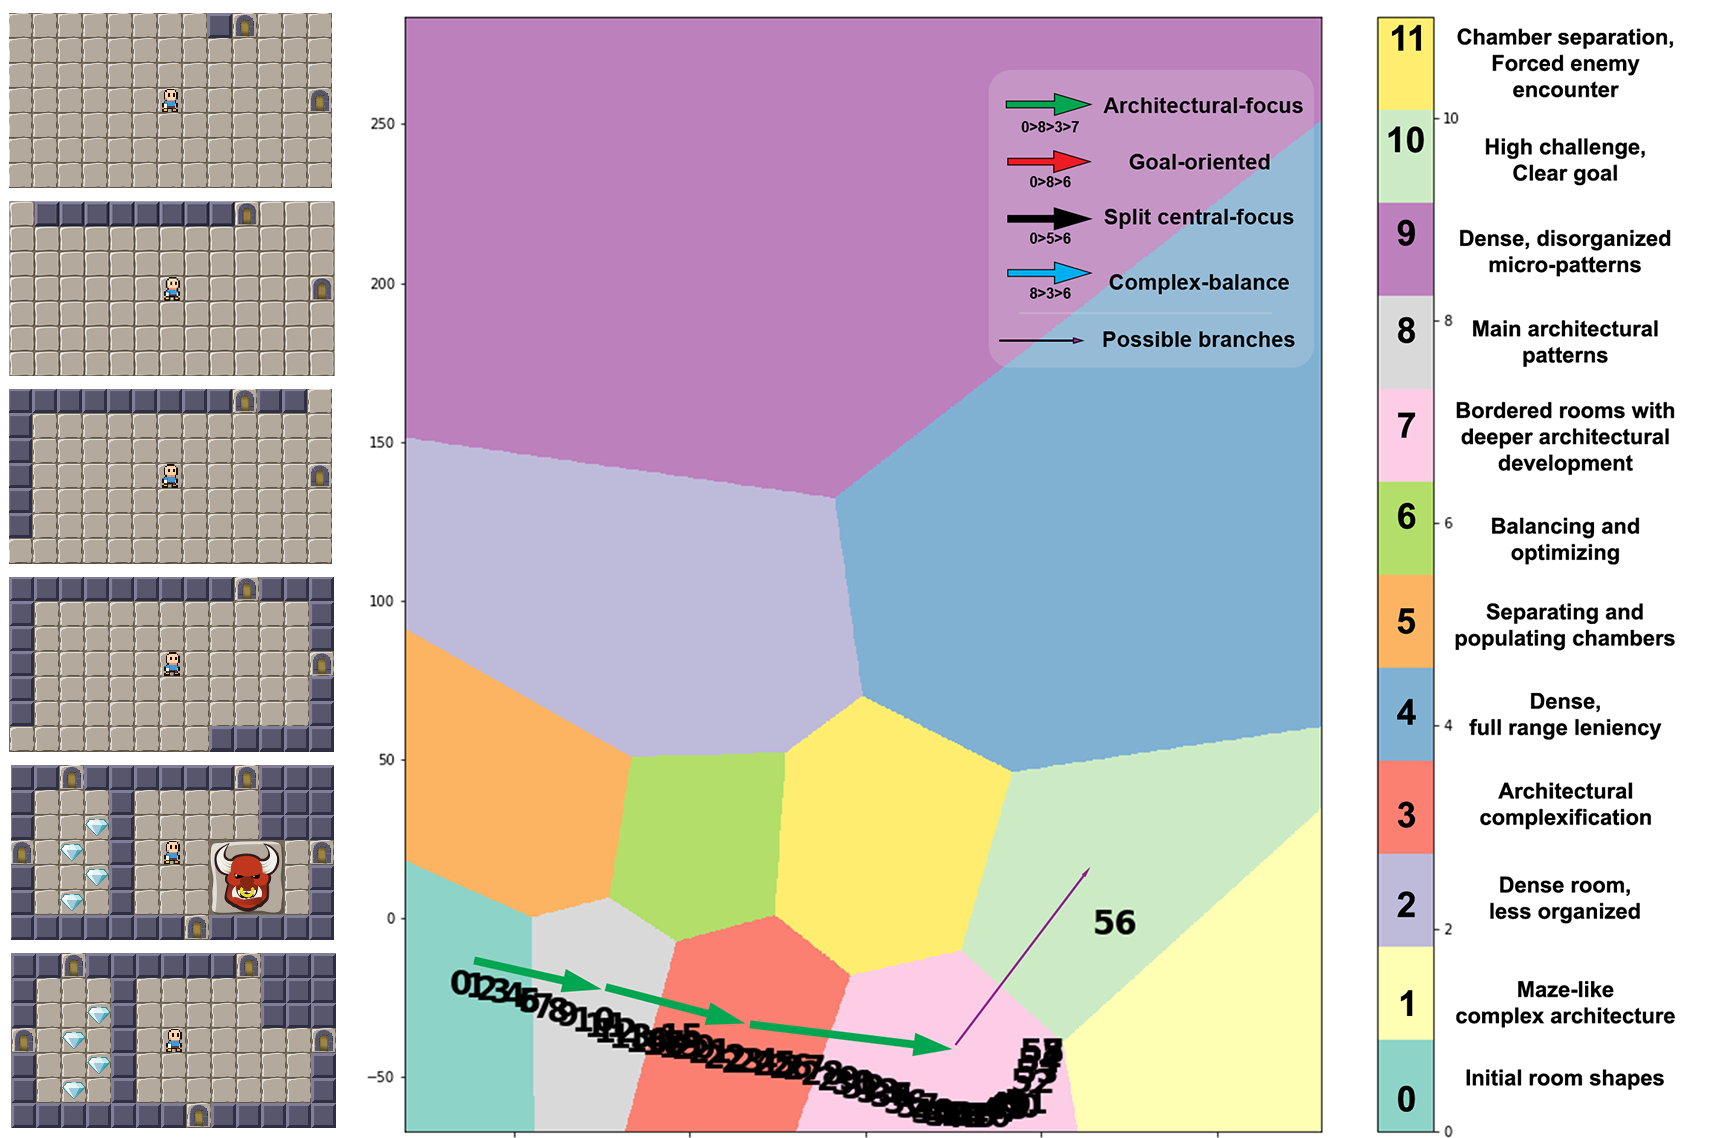
\includegraphics[width=0.45\textwidth]{figures/1.png}
     }
     \hfill
     \subfloat[\textsc{Goal-oriented}\label{p6subfig-2:dummy}]{%
       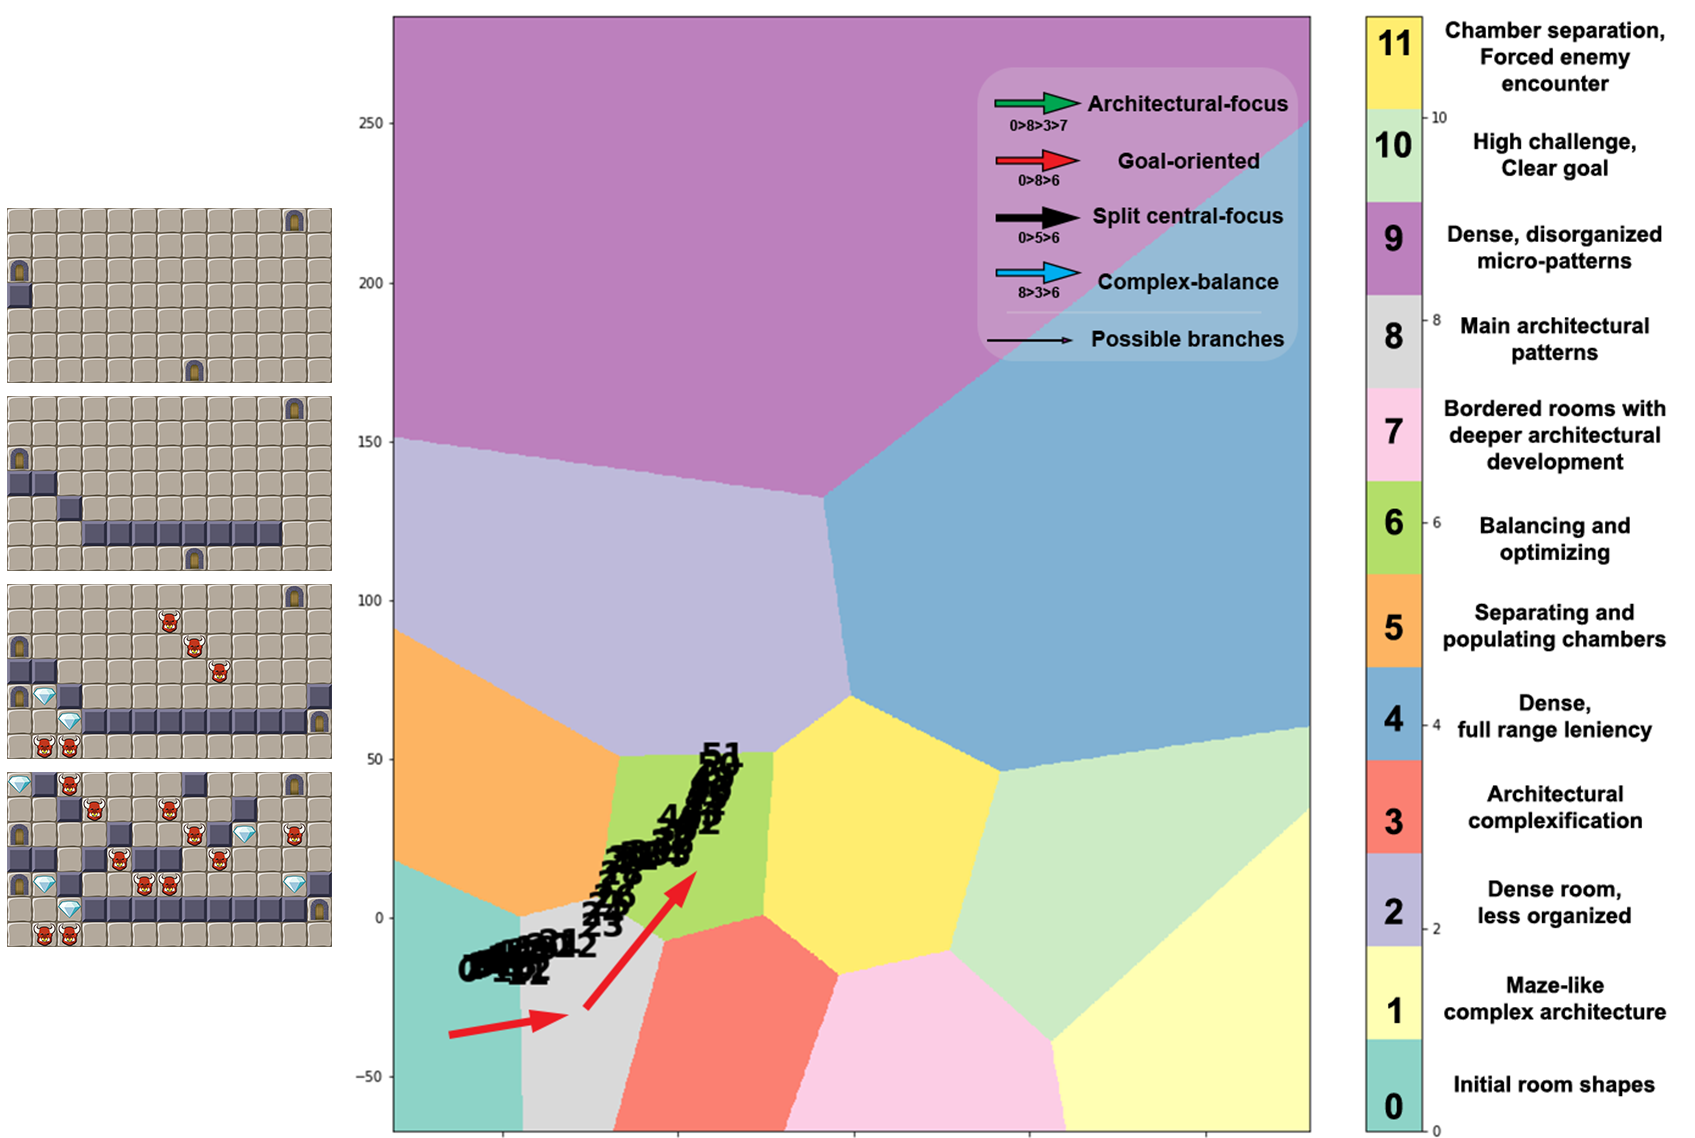
\includegraphics[width=0.45\textwidth]{figures/2.png}
     }\hfill
    %  \medskip
     \subfloat[\textsc{Split central-focus}\label{p6subfig-3:dummy}]{%
       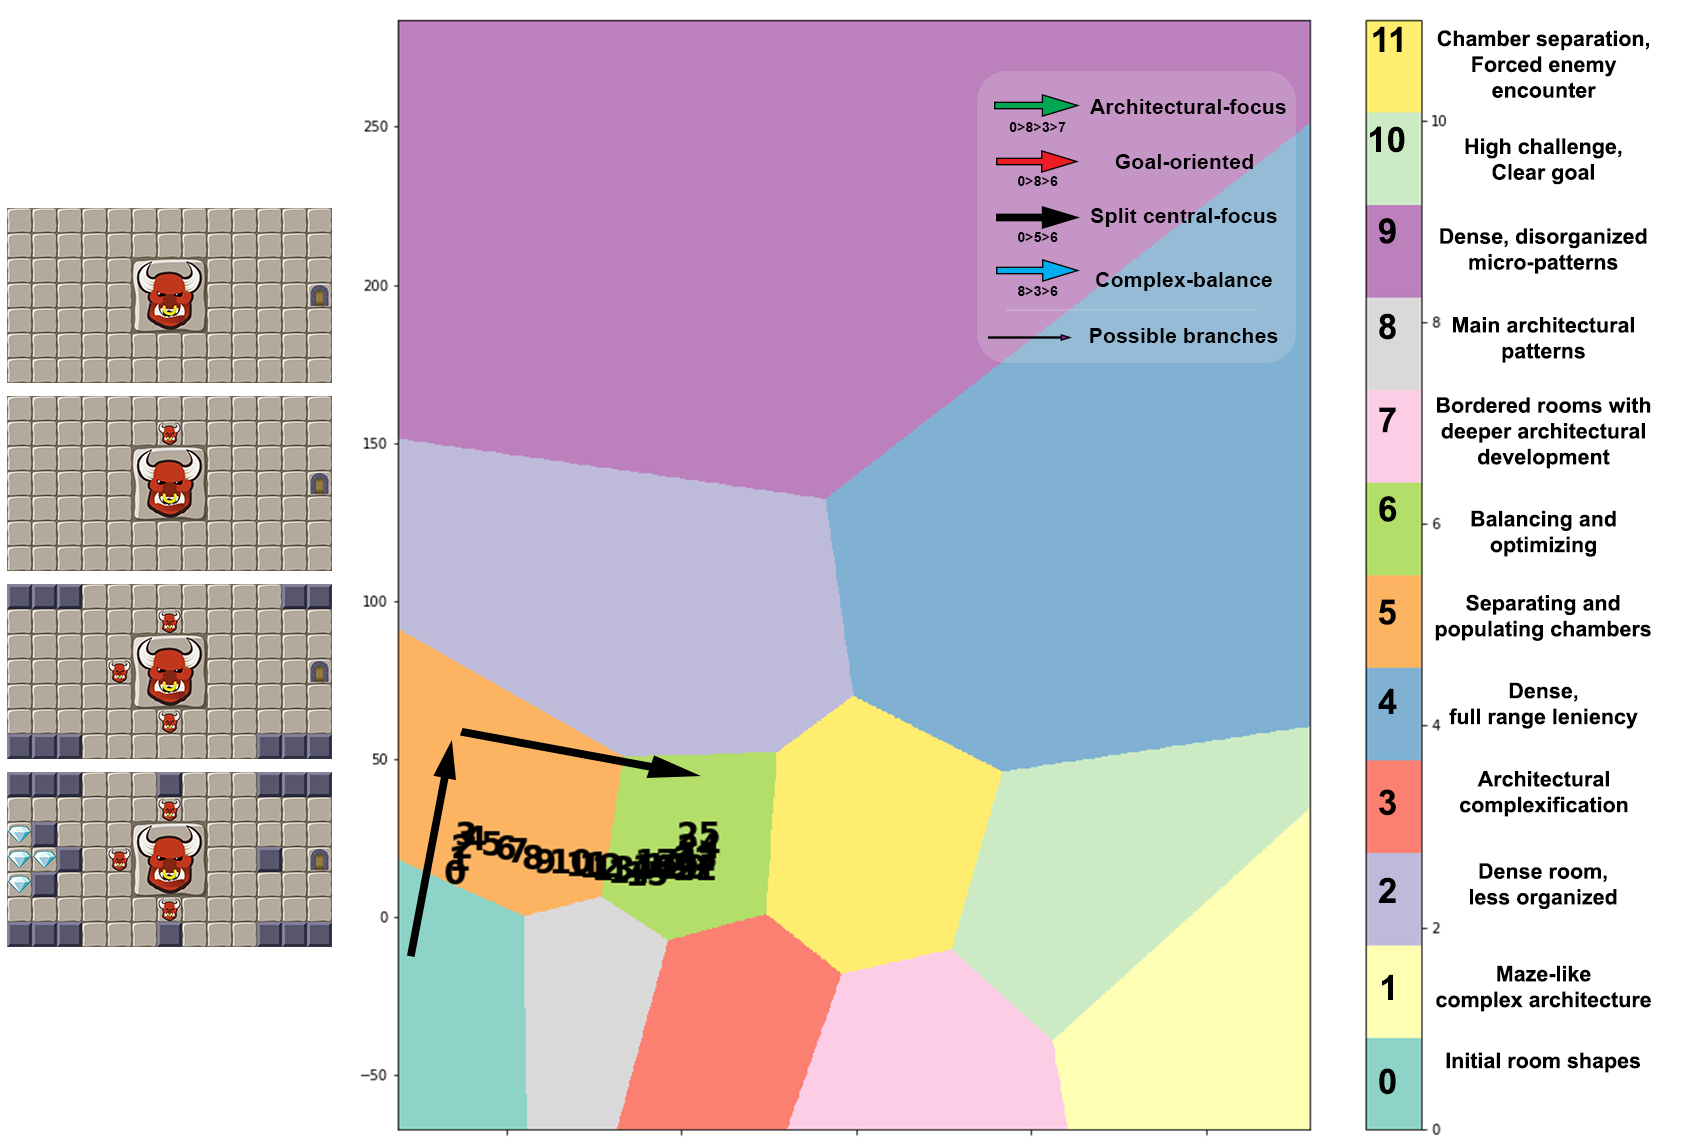
\includegraphics[width=0.45\textwidth]{figures/3.png}
     }
     \hfill
     \subfloat[\textsc{Complex-balance}\label{p6subfig-4:dummy}]{%
       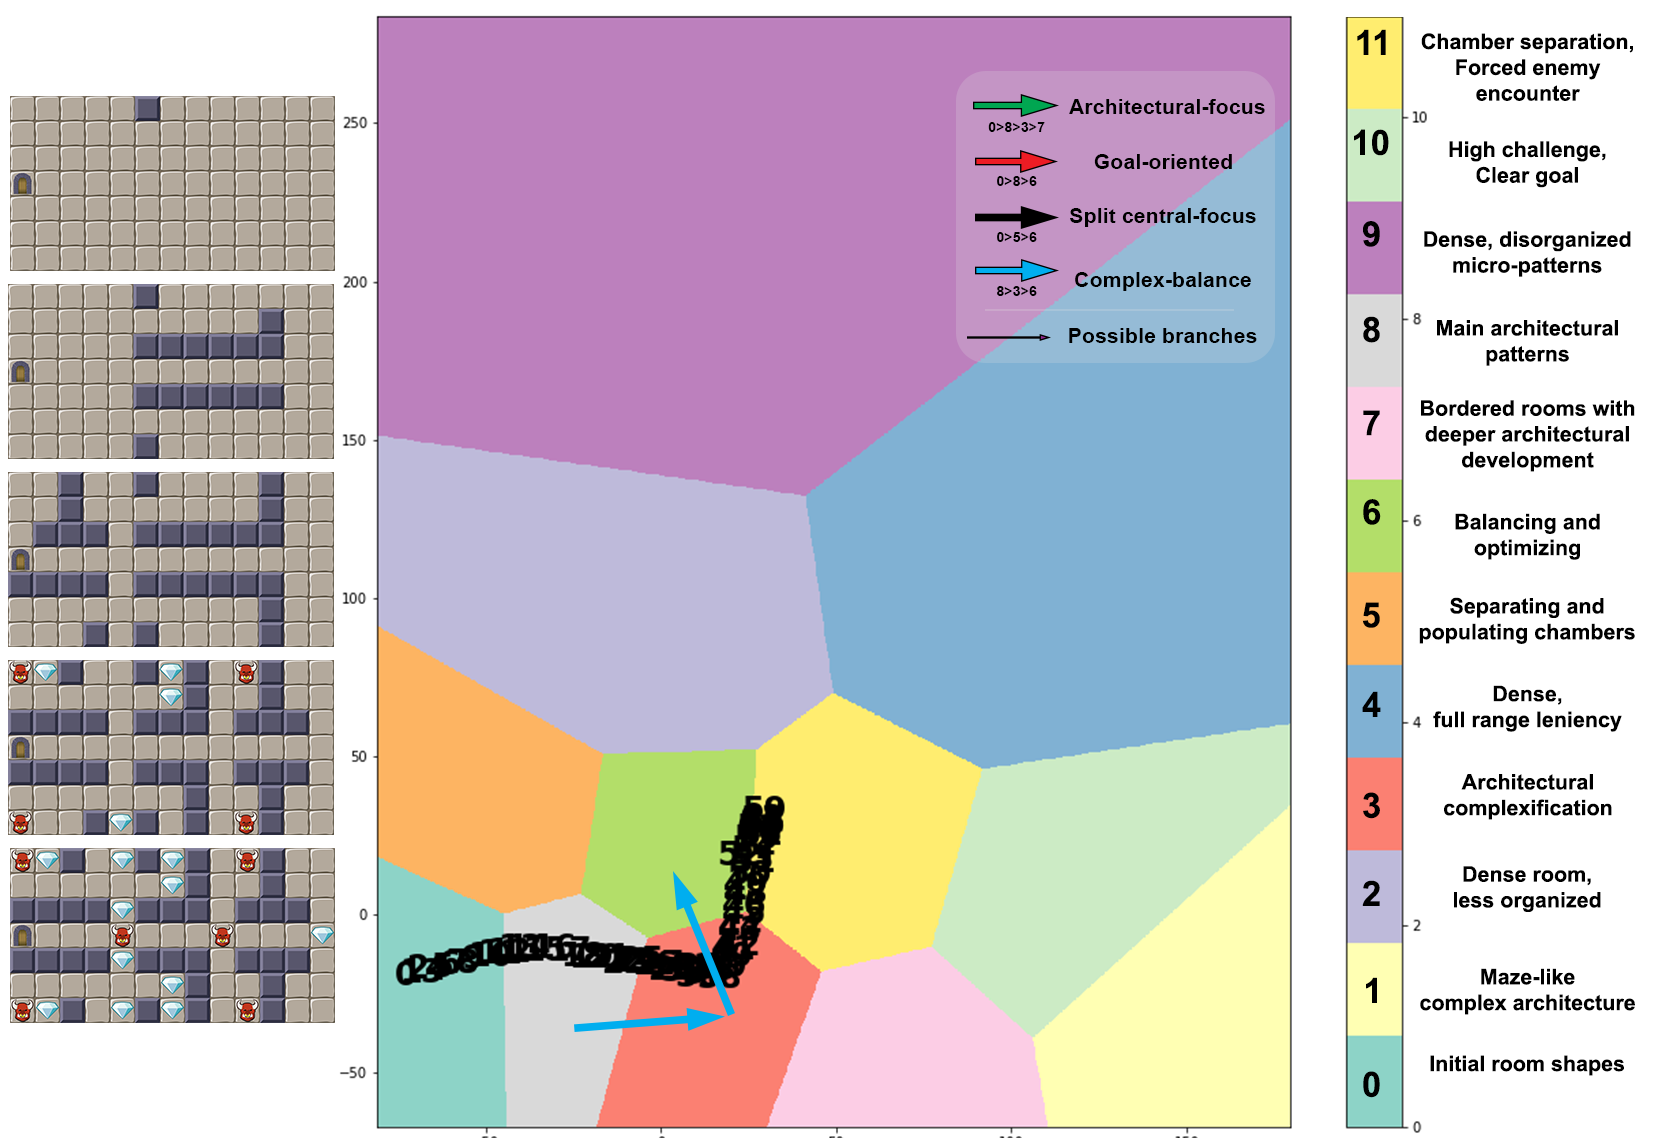
\includegraphics[width=0.45\textwidth]{figures/4.png}
     }
    
    \caption{Examples of each of the archetypical paths from one of the frequent sequences used to create the clusters. To the left of each subfigure, we present each key step in the trajectory i.e. when the design entered a new cluster. (a) presents the \textsc{Architectural-focus} archetypical path where the focus is firstly on creating the structural design of the rooms; the design process jumps back and forth suddenly to cluster 10 (one of the possible branches) due to the designer adding a boss, and removing it immediately. (b) presents the \textsc{Goal-oriented} archetypical path where the design focus on a minimal structure complexity and mix between adding structural changes and enemies/treasures. (c) shows the \textsc{Split central-focus} archetypical path where, intentionally, the designer creates a center obstacle with a boss and build around it. Finally, (d) presents the \textsc{Complex-balance} archetypical path; the design focuses on building complex, uncommon structures first and then add some goal to it with enemies and treasures, taking advantage of the spaces.}
    \label{p6fig:archetypical-examples}
\end{figure*}


Once we created, evaluated, and labeled the clusters, we were able to cluster and visualize the paths of a typical design session. Figure \ref{p6fig:paths-designers} presents an example of the design sessions, where we cluster each step of the design. This sequential process revealed that there is an interesting continuity between clusters, even capturing when a designer probably applied one of the procedural suggestions due to bigger steps in the design style clusters. Further, through this process, we could understand the progress of designers in their design process and represent their trajectory in relation to the traversed clusters rather than individual editions.

\subsubsection{Unique Trajectories}

Using the clusters in Figure \ref{p6fig:all-clusters}, we clustered the design session of all the $180$ designs and collected the unique trajectories that arose from traversing the various clusters. These unique trajectories varied in the starting point, length, and end-point, however, when analyzing the trajectories we identified common patterns among them. They had a similar shape as the following $Unique=$\{0\textgreater8\textgreater4\textgreater7\textgreater10\}, where the first and last element of the sequence are respectively, the starting- and end-points, with all the unique intermediate steps in between.

To gather the common patterns from the trajectories, we applied the Generalized Sequential Pattern (GSP) algorithm, which locates frequent subsequences in the analyzed trajectories. For instance, given three trajectories (a) \{5\textgreater1\textgreater3\textgreater11\textgreater9\}, (b) \{5\textgreater1\textgreater3\textgreater11\textgreater4\, and (c) \{0\textgreater1\textgreater3\textgreater11\}, none of these is a perfect match in its entirety, but GSP can spot that subsequences \{1\textgreater3\textgreater11\}, \{1\textgreater3\}, \{3\textgreater11\}, among others, appear with frequency $= 3$.

%(2) obtain only 1 pattern ($\{5>1>3>11\}$) with frequency=2, if searching from starting points. Finally, using GSP, we find $\{5>1>3>11\}$, $\{1>3>11\}$, $\{1>3\}$, $\{3>11\}$

%We collected these unique trajectories, and 
Furthermore, after doing a preliminary analysis, we identified some steps that we classified as ``border designs'': steps that are borderline between two clusters. These \textit{border designs} disrupted the sequence pattern mining by creating noise in the unique trajectories, specifically when these \textit{border designs} entered a different cluster for just a few steps. %we categorize them as when these "unique" noisy steps were brief.
Therefore, we filtered them out by applying a threshold $\theta = 3$, so that all subsequences inside one cluster with less than $\theta$ steps are removed from the main sequence. I.e, the sample trajectory \{0\textgreater0\textgreater0\textgreater0\textgreater8\textgreater8\textgreater8\textgreater6\textgreater8\} turns into \{0\textgreater8\} instead of \{0\textgreater8\textgreater6\textgreater8\}. Through this, we were able to reduce the noise and the search space, obtaining more meaningful and frequent patterns.

\subsubsection{Archetypical Paths through Style Space}

%Figure \ref{p6fig:finalPaths} shows the archetypical paths taken by designers when creating rooms. Represented as arrows to denote direction, 

%From all the collected unique trajectories, we identified 4 main archetypical paths, which are the ones taken most frequently by designers either as their full path or as the initial path. In Figure \ref{p6fig:finalPaths}, it is shown the archetypical paths, represented as thicker arrows to denote direction, that represent the taken by designers when creating rooms. 

In Figure \ref{p6fig:finalPaths}, we present the archetypical paths, represented as thicker arrows to denote direction, which show the most frequent paths taken by designers either through their whole design process or as the initial meaningful steps. From all the collected unique trajectories, we have identified 4 main archetypical paths, labelled, \textsc{Architectural-focus}, \textsc{Goal-oriented}, \textsc{Split central-focus}, and \textsc{Complex-balance}. In addition, we have numbered each cluster for easier visualization and referencing. 

Moreover, in the figure, it can also be observed thinner purple arrows pointing to different clusters from several of the clusters that are part of the main paths. These are \textit{possible branches} presented in the unique trajectories and added based on their frequency. Through these possible branches, the design of an archetypical session, can vary and extended or deviate the final design. Each archetypical path is defined and explained as follows: 

\paragraph{Architectural-focus}The path followed by this archetype focuses first on designing the architecture of the room with walls. Through this, the design focuses on shaping the visual patterns, chambers, and corridors to give a clear space for adding goals and objectives with enemies and treasures. The sequence is denoted with a green arrow in Figure \ref{p6fig:finalPaths}, and following the sequence \{0\textgreater8\textgreater3\textgreater7\}.

\paragraph{Goal-oriented}Design processes following this archetypical path, create the rooms in a more standard way, combining simpler symmetric wall structures with distributed placement of enemies and treasures. Thus, rather than focusing extensively on an individual part of the room, the rooms have an initial structure and then they are populated with some specific goal-in-mind. The sequence is denoted with a red arrow in Figure \ref{p6fig:finalPaths}, and following the sequence \{0\textgreater8\textgreater6\}.

%Thus, rather than focusing on an individual part of the room until satisfied, the rooms have some initial structures that are populated and continue through an iterative process between these steps.% rooms go through an iterative process of adding have some initial structures that are

\paragraph{Split central-focus}This archetypical path focuses on designing rooms with obstacles placed in the center of the room in the shape of enemies, treasures, or wall structures that clearly split the room into different areas. The design process is less organized than the other archetypes since it searches to achieve the split goal with any of the available tiles. The sequence is denoted with a black arrow in Figure \ref{p6fig:finalPaths}, and following the sequence \{0\textgreater5\textgreater6\}.
%, since the middle step is cluster 5 ("Separating and populating chambers"), which relates to rooms which are expected since the cluster 5 ("Separating and populating chambers") relate to rooms that  as specific structural shapes are not necessary. 

\paragraph{Complex-balance}This archetypical path focuses on building complex symmetric shapes with a clear objective for the player and adapting the spaces with a balance of enemies and treasures. In general, the rooms created following this path are more unique and typically balanced. %   with that adapt well. The process is quite 
The sequence is denoted with a blue arrow in Figure \ref{p6fig:finalPaths}, and following the sequence \{8\textgreater3\textgreater6\}.

Furthermore, using these archetypical paths, we can then categorize certain clusters as key clusters or being more relevant than others based on their contribution to the paths, their frequency, and their usage. Most of the paths go through or end in cluster 6 (``Balancing and optimizing'') and cluster 8 (``Main architectural patterns''), which relate to rooms that have a more explicit mix between corridors and small chambers and more clear architecture. The rooms in those clusters are or shaped as end rooms, as in the case of cluster 6, or architecturally shaped to be “optimized” to a specific goal e.g. a dense bordered room. Similarly, most of the sequences start from cluster 0 ("Initial room shapes"), with $134$ out of the $180$ designs, which correlates to the type of designs encountered in that clusters. Thus, it is understandable that most of the archetypical paths pass through any of these three clusters. 

Nevertheless, it is the steps in-between what creates a clear differentiation between the archetypical paths, which is the benefit of observing the design process as a whole in the clustered room style space. For instance, in fig.~\ref{p6fig:finalPaths}, it can be observed that \textsc{Split central-focus} starts in the same cluster as three other paths, and tentatively ends in the same cluster as three other. However, the designs following \textsc{Split central-focus} are more different to the other trajectories, since it enters a cluster that is denser with several tile types in principle, and where designers seem to have a clearer goal.
% With this, we can further understand why \textsc{Split central-focus} is more different to the other trajectories, since it enters a cluster that is "less organized" in principle. 

%Furthermore, we can also observe that certain clusters are key steps for most paths because they are or a frequent starting or ending point. Most of the paths go through or end in cluster 6 ("Balancing and optimizing") and cluster 8 ("Main structural patterns"), which relate to rooms that have a more explicit mix between corridors and small chambers and a more clear structure, thus, it is understandable since the rooms in those clusters are or shaped as end rooms, as in the case of cluster 6, or structurally shaped to be “optimized” to a specific goal (E.g. dense bordered room, maze-like, more challenging, etc.). However, the distribution of endpoints is quite even, and meanwhile, cluster 6 and cluster 11 ("Chamber separation, Forced enemy encounter") are the most frequent ending points with $36$ and $25$ out of $180$ design processes, the rest of clusters are quite close.

%Similarly, most of the sequences start from cluster 0 ("Initial room shapes"), with $134$ out of the $180$ designs, which correlates to the type of designs encountered in those clusters.

Moreover, in figure~\ref{p6fig:archetypical-examples}, we present examples of each of the designer personas by visualizing the sequence of steps done in representative design sessions, showing how these paths would look like in practice. Each visualization of a designer persona has the key design steps to the left, where each image is in a sequence: the first is the first edition of the designer, the last is the final edition, and the in-between represent entering a new room style cluster. 

In (a), it is shown the \textsc{Architectural-focus}, where the designer first created the border of the room with a clear chamber division. As the designer adds and subsequently removes the boss, the design jumps to cluster 10, which is one of the possible branches, adding a high challenge. In (b), it is shown the \textsc{Goal-Oriented}, where the designer sketched the main shape of the room followed by alternating between enemies, treasures, and walls to design the goal of the player within the room. In this example, the designer ends the design close to cluster 9, with a disorganized placement of tiles and a less aesthetical room, but forming small choke areas balancing the placement of enemies and treasures.

In (c), it is shown the \textsc{Split Central-focus}, where the designer directly started by adding a boss in the center of the room and using this as a reference point, shaped the rest of the room. In (d), it is shown the \textsc{Complex-balance}, where the designer focused on creating an uncommon structure and followed by adding enemies and treasures symmetrically, with clear individual areas for the player to approach.

% It is not surprising to focus on the center as it 

Finally, further analyzing figure~\ref{p6fig:archetypical-examples}, it can also be observed an interesting dual tendency of the designers in the archetypical paths. This dual tendency is to either focus on the aesthetic configuration of the room based on what is perceived in the editor exemplified the personas: \textsc{Architectural-focus} and \textsc{Split central-focus}, and to focus on the player experience exemplified the personas: \textsc{Goal-oriented} and \textsc{Complex-balance}. Nevertheless, both are not mutually exclusive, instead this illustrates adequately the dualistic role the designer has when using the tool and designing rooms. That of creating an aesthetically pleasing object as it is seen in the editor, and that of creating an experience.% However, this is not mutually exclusive. Instead, it shows 


% Furthermore, when analyzing how the different design sequences were clustered and forming the designer personas, we observed an interesting dual tendency of the designers. This dual tendency is to either focus on the aesthetic configuration of the room based on what is perceived in the editor through the personas: \textsc{Architectural-focus} and \textsc{Split central-focus}, and to focus on the player experience through the personas: \textsc{Goal-oriendted} and \textsc{Complex-balance}. This exemplified quite good 
% dualistic role 
% When forming the designer personas, and analyzing how different design sequences


%where the designer focused on creating the shape of the room before adding any enemyfirst created the border of the room

% Finally, in Figure \ref{p6fig:archetypical-examples}, we present examples of each of the archetypical paths to show how would these paths look like in practice, further supporting our findings and path definitions. 

% The archtypical paths a dual tendency of the designers to either go for a strategy that reflects their perception of the level from the editor - like the aesthetic configurations of it, instead of the experiential ones. for example the ones that had a split central focus and a structural focus (which btw maybe i would change to architectural focus). and then there's the ones that have a focus on the player experience like the goal oriented and complex behavior ones. i think this split reflex a very nice dualistic role that the designer has in front of the editor - that of creating an aesthetically pleasing object, as they see it in the editor, and that of creating an experience.
% , and exmplified
%That build around



% Notice that not all the clusters have connectionthat based on the unique trajectories, where designers decided to move towards other areas. 

%it is shown the archetypical paths, represented as thicker arrows to denote direction, that represent the taken by designers when creating rooms. 
% moving from 6 to 11 or from 3 to 11 is a fairly frequent step, thus making it and cluster 6, key points.
% In fact, ending the design at 7 is not that common, thus, 



% the red cluster with $95$ out of the $180$, and from the purple cluster with $49$ out of the $180$, which correlates to the type of designs encountered in those clusters, mainly emptier rooms with initial sketches and shapes. 

% Most of the paths start in cluster 0 ("Initial room shapes") 

% From the figure, we can extract the following clusters as key steps for most of the patterns: "light green", "light blue", "red", and "purple". 

% It can be observed that most of the paths end or go through the "light green" and "light blue" clusters. Both relate to rooms that have a more clear structural pattern and more explicit mix between corridors and small chambers, thus, is understandable since the rooms in those clusters are or shaped as end rooms or structurally shaped to be “optimized” to a specific goal (E.g. dense bordered room, maze-like, more challenging, etc.). Quantitatively, most of the sequences end up in those clusters, $64$ out of the $180$ end in cluster 6 (light blue) and $52$ out of the $180$ end in cluster 11 (light green).


% Similarly, most of the sequences start from the red cluster with $95$ out of the $180$, and from the purple cluster with $49$ out of the $180$, which correlates to the type of designs encountered in those clusters, mainly emptier rooms with initial sketches and shapes. 


% \begin{figure*}
% \centerline{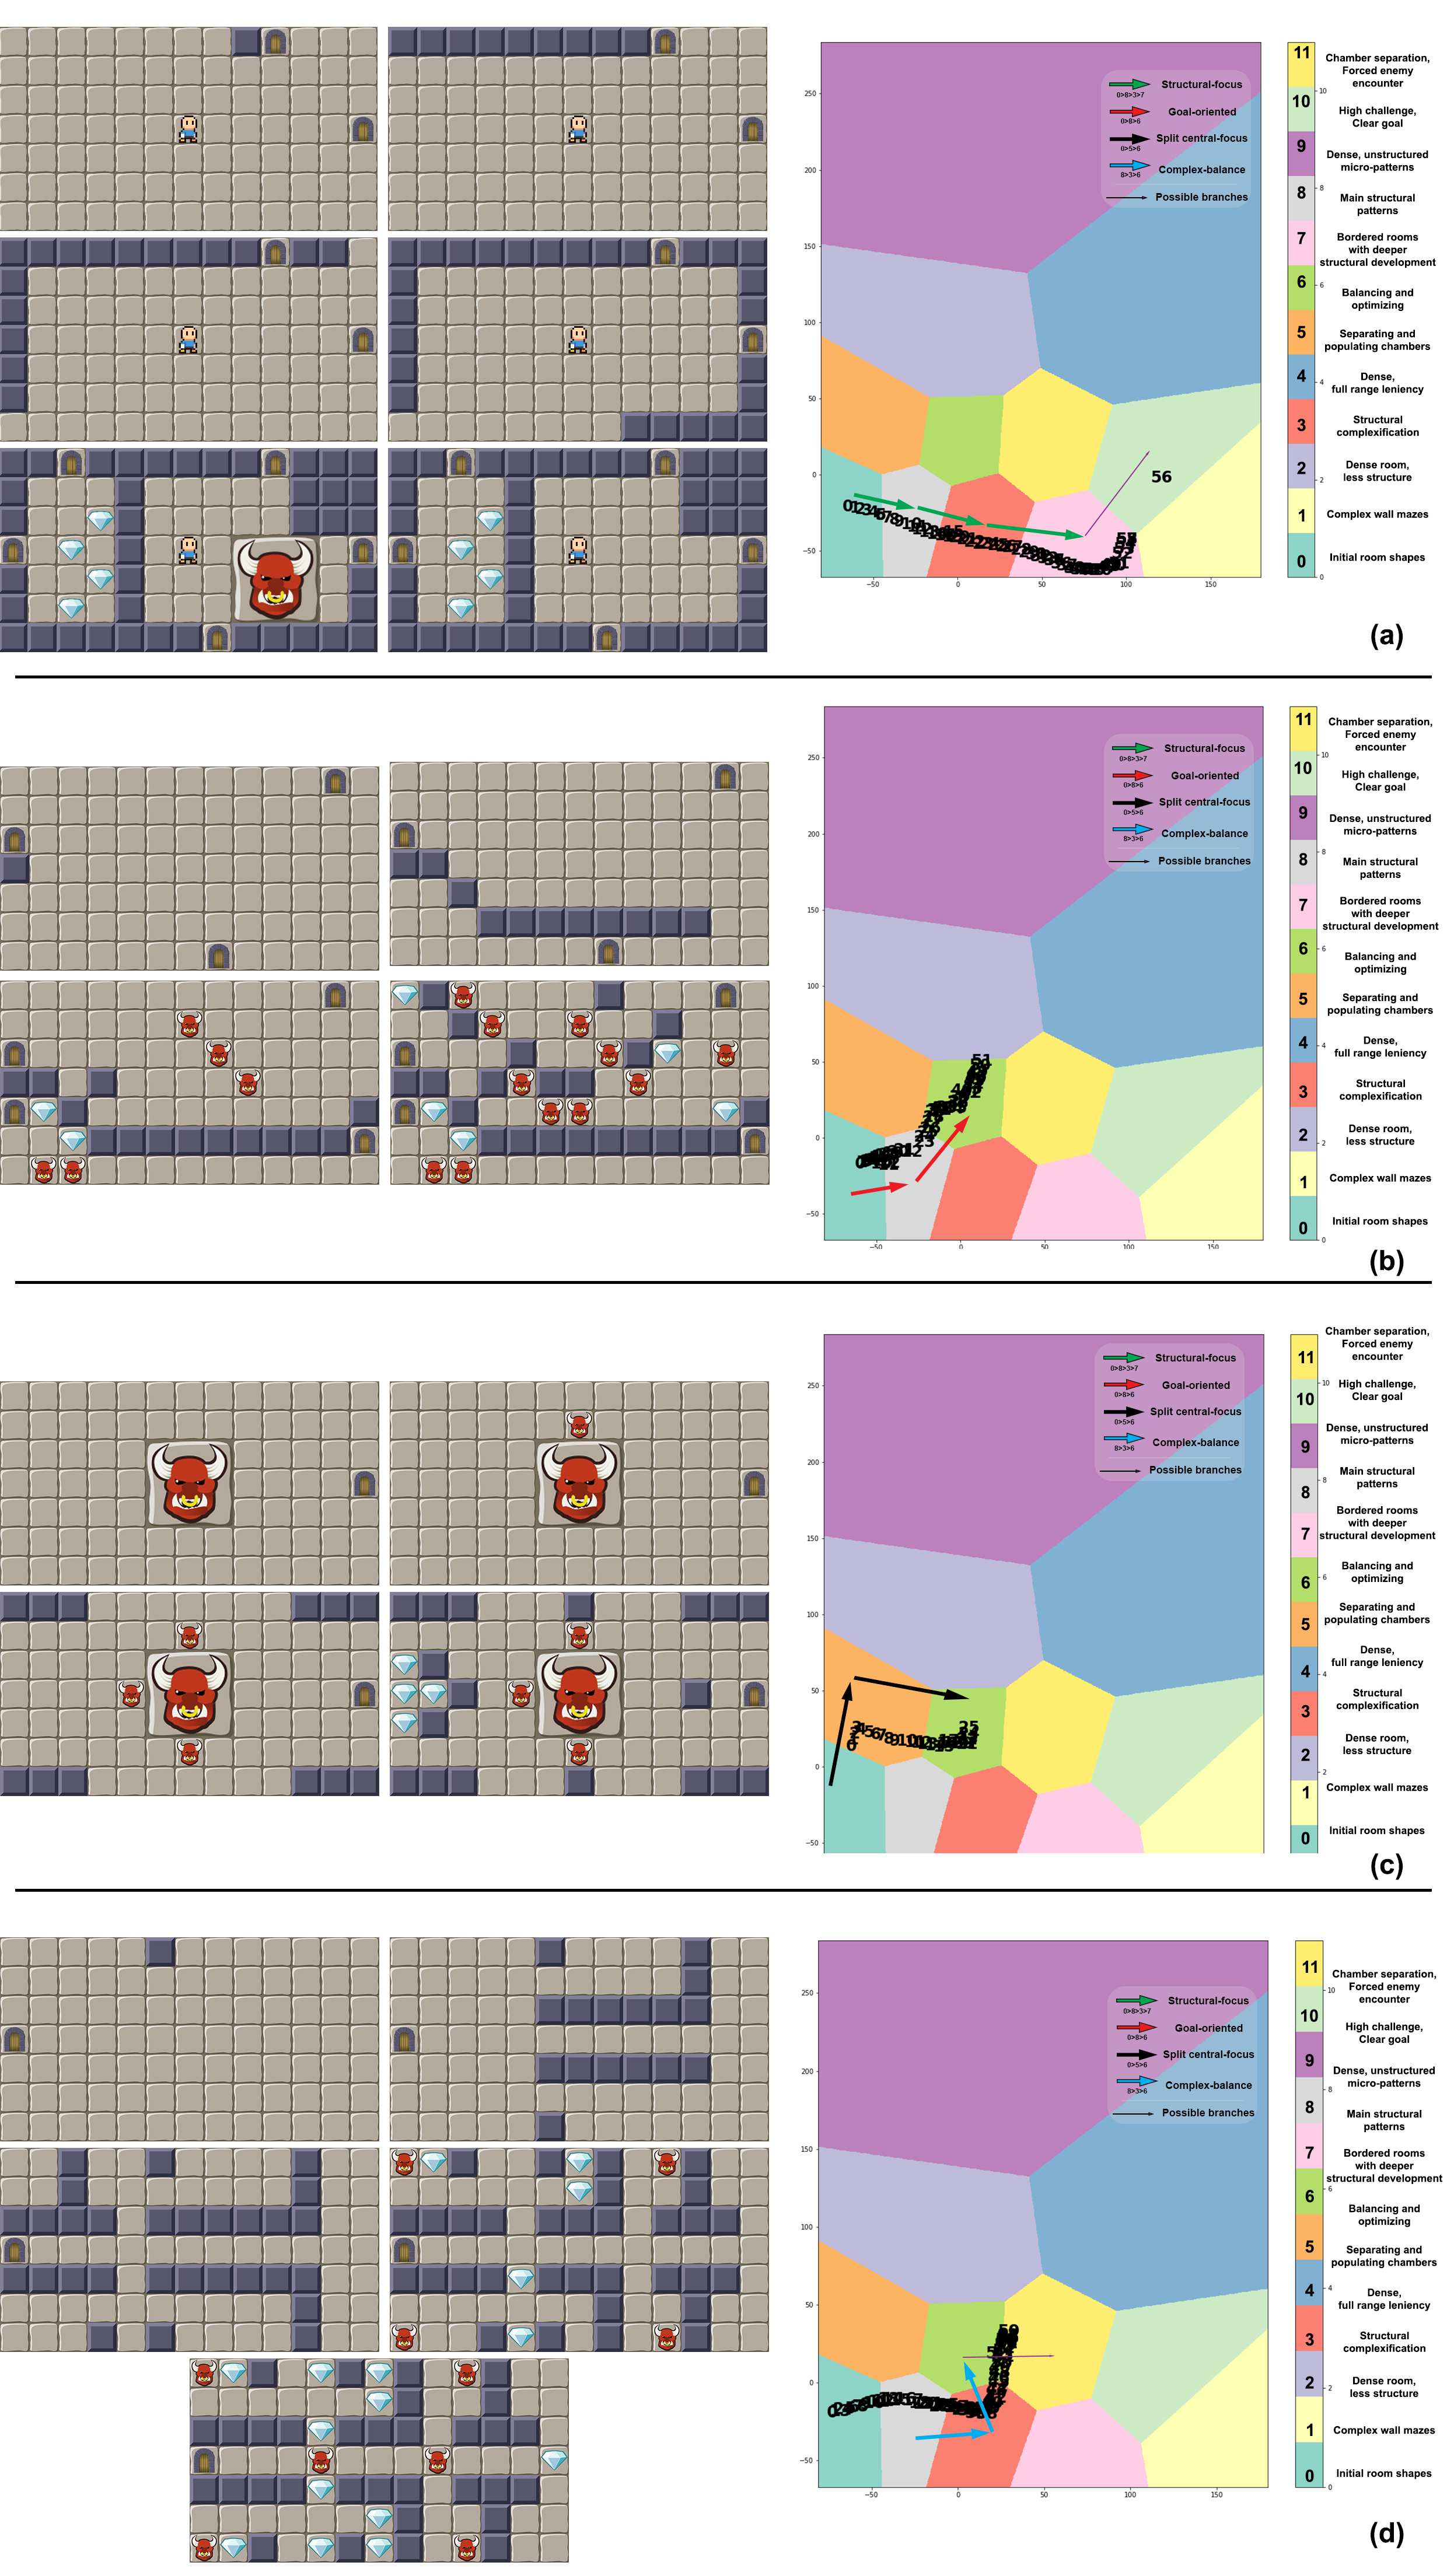
\includegraphics[width=0.7\textwidth]{figures/path-examples-2.png}}
% \caption{Examples of each of the archetypical paths from one of the frequent sequences used to create the clusters. To the left of each subfigure, we present each key step in the trajectory i.e. when the design entered a new cluster. (a) presents the \textsc{Structural focus} archetypical path where the focus is firstly on creating the structural design of the rooms; the design process jumps back and forth suddenly to cluster 10 (one of the possible branches) due to the designer adding a boss, and removing it immediately. (b) presents the \textsc{Goal-oriented} archetypical path where the design focus on a minimal structure complexity and mix between adding structural changes and enemies/treasures. (c) shows the \textsc{Split central-focus} archetypical path where intentionally, the designer creates a center obstacle with a boss and build around it. Finally, (d) presents the \textsc{Complex-balance} archetypical path; the design focuses on building complex uncommon structures first and then add some goal to it with enemies and treasures, taking advantage of the spaces.} \label{p6fig:archetypical-examples}
% \end{figure*}



% \begin{subfigure}[t]{0.33\textwidth}
%         \centering
%         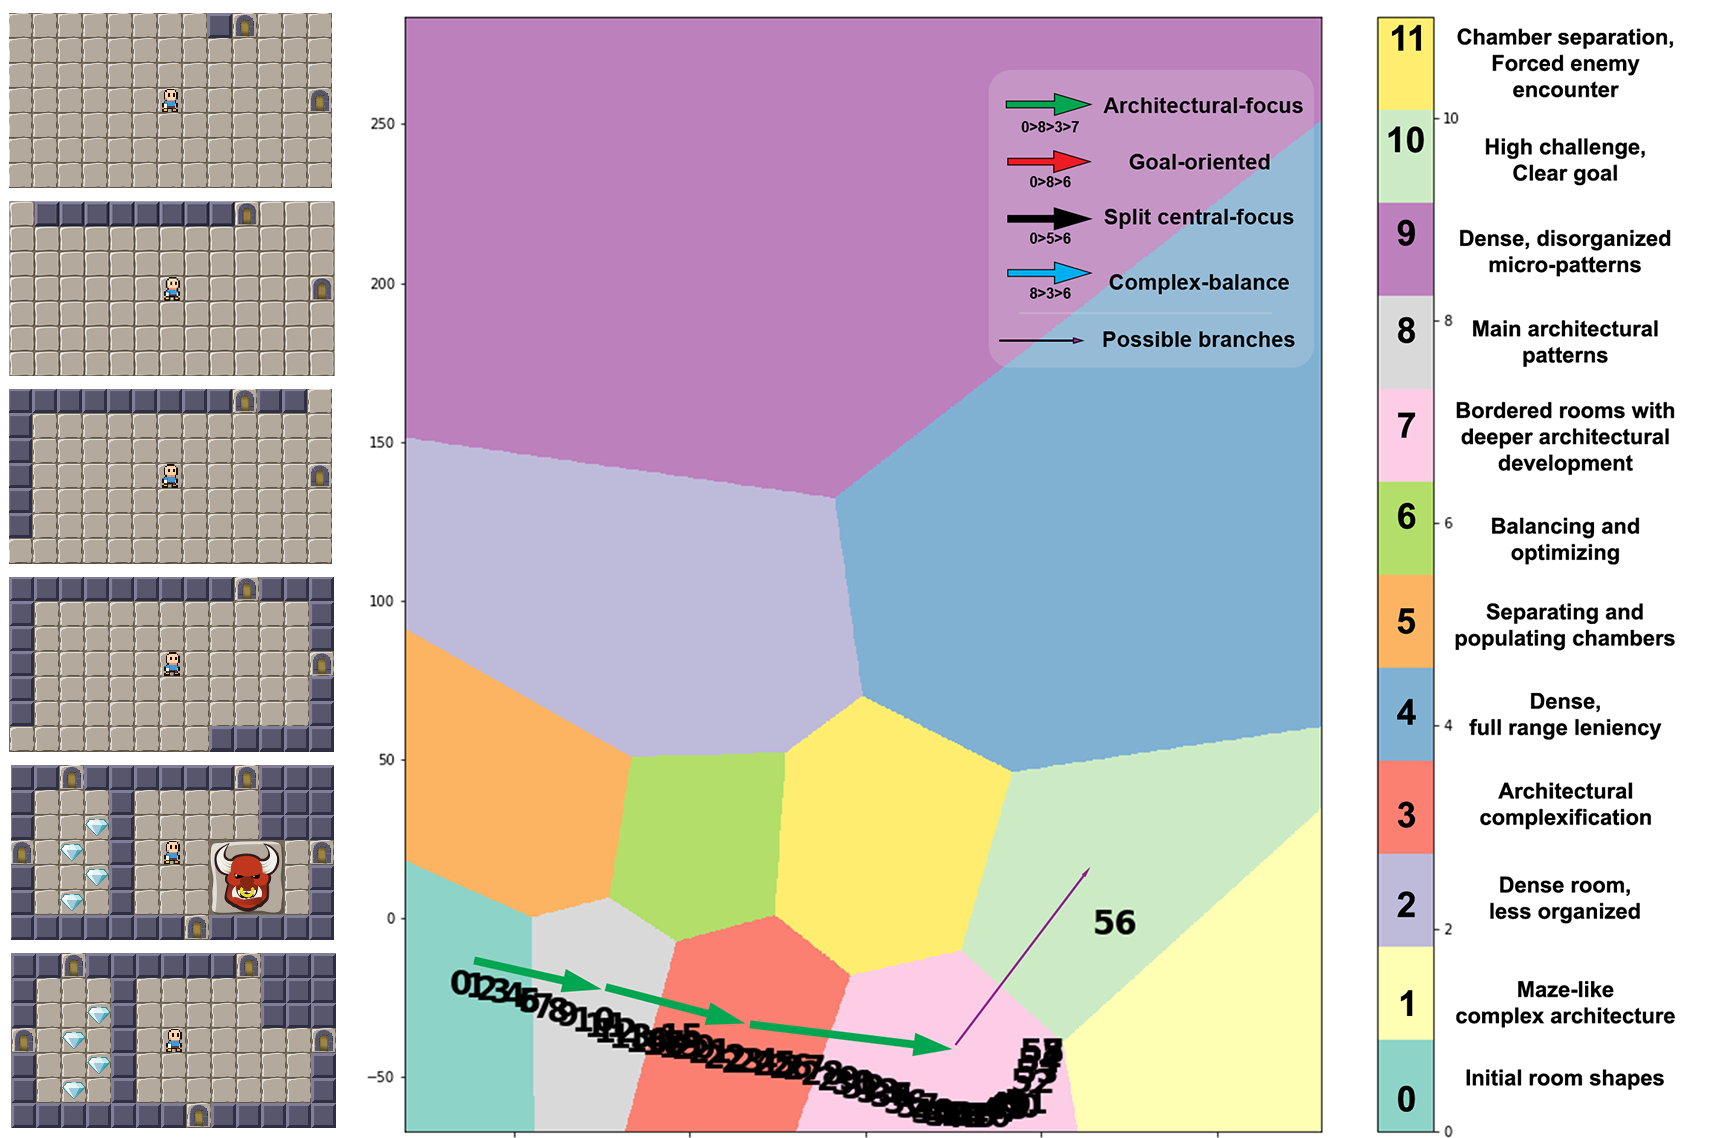
\includegraphics[width=0.95\textwidth]{figures/1.png}
%         \caption{Linearity-\#MesoPatterns}
%     \end{subfigure}%
%     \begin{subfigure}[t]{0.33\textwidth}
%         \centering
%         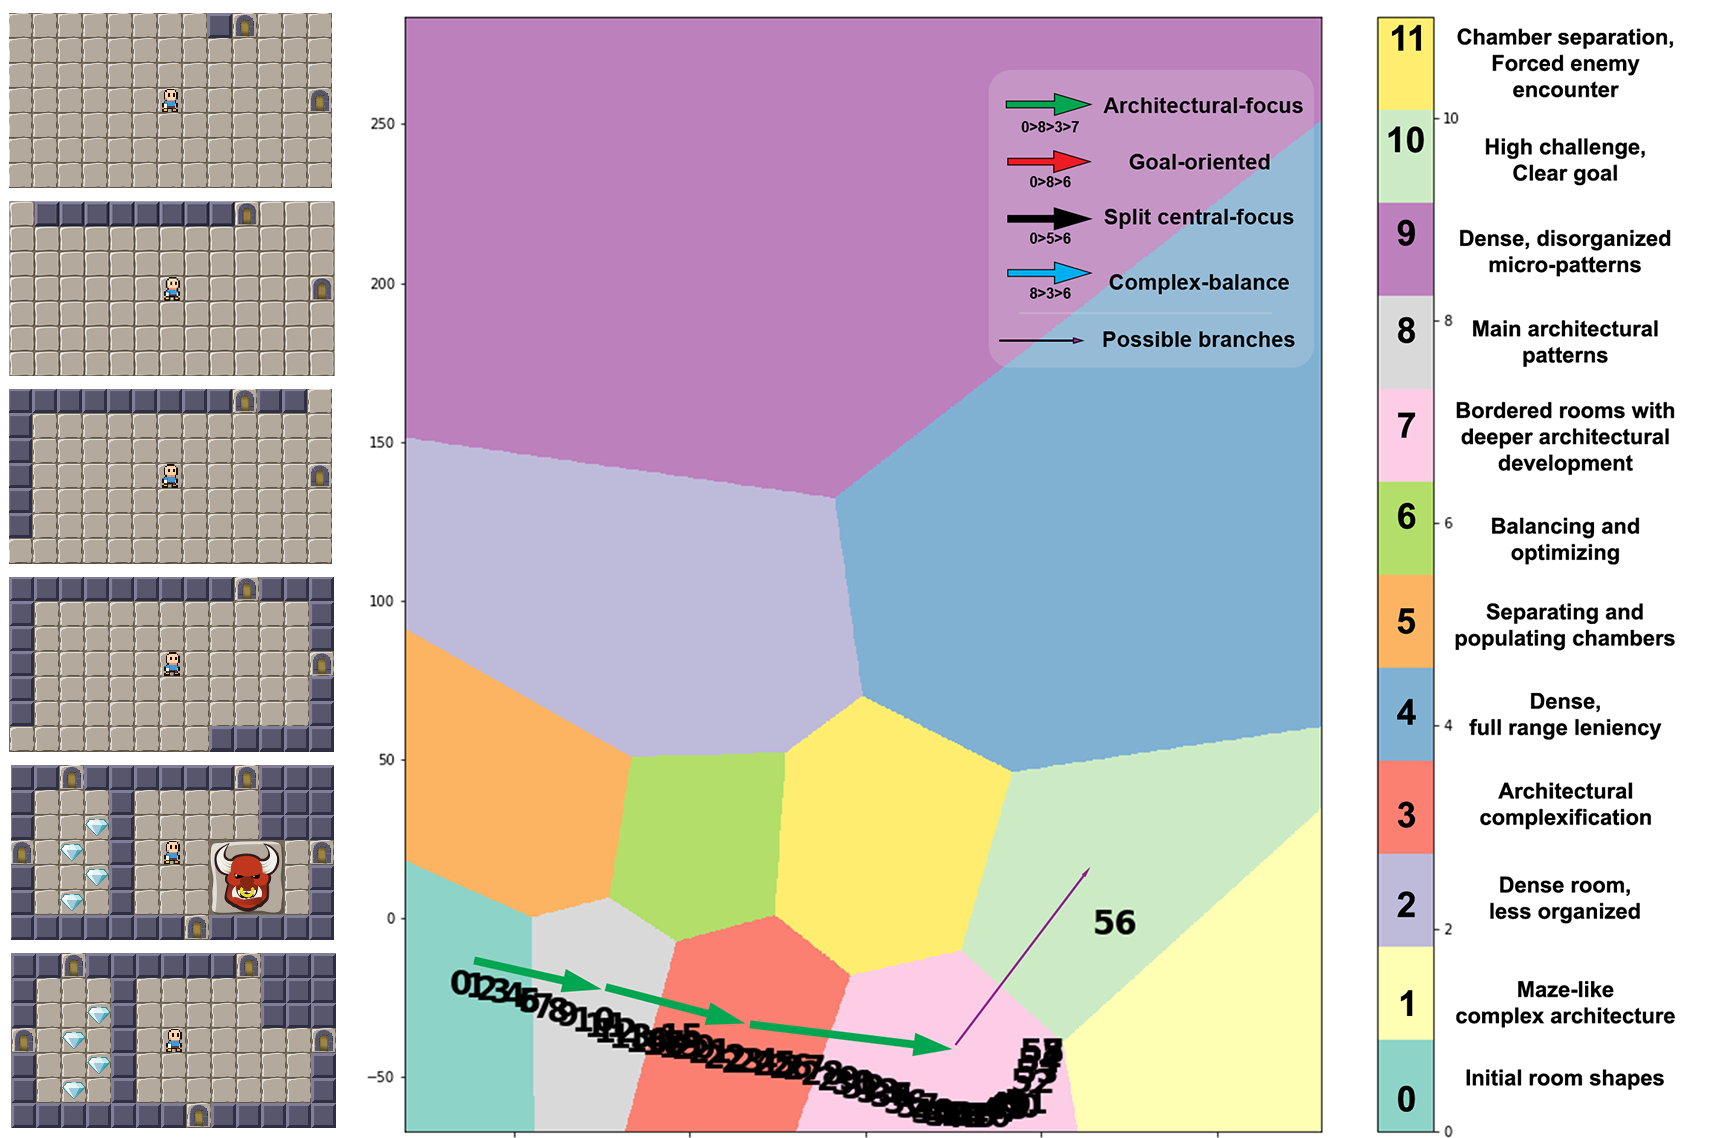
\includegraphics[width=0.95\textwidth]{figures/1.png}
%         \caption{Linearity-\#MesoPatterns}
%     \end{subfigure}%
%     \begin{subfigure}[t]{0.33\textwidth}
%         \centering
%         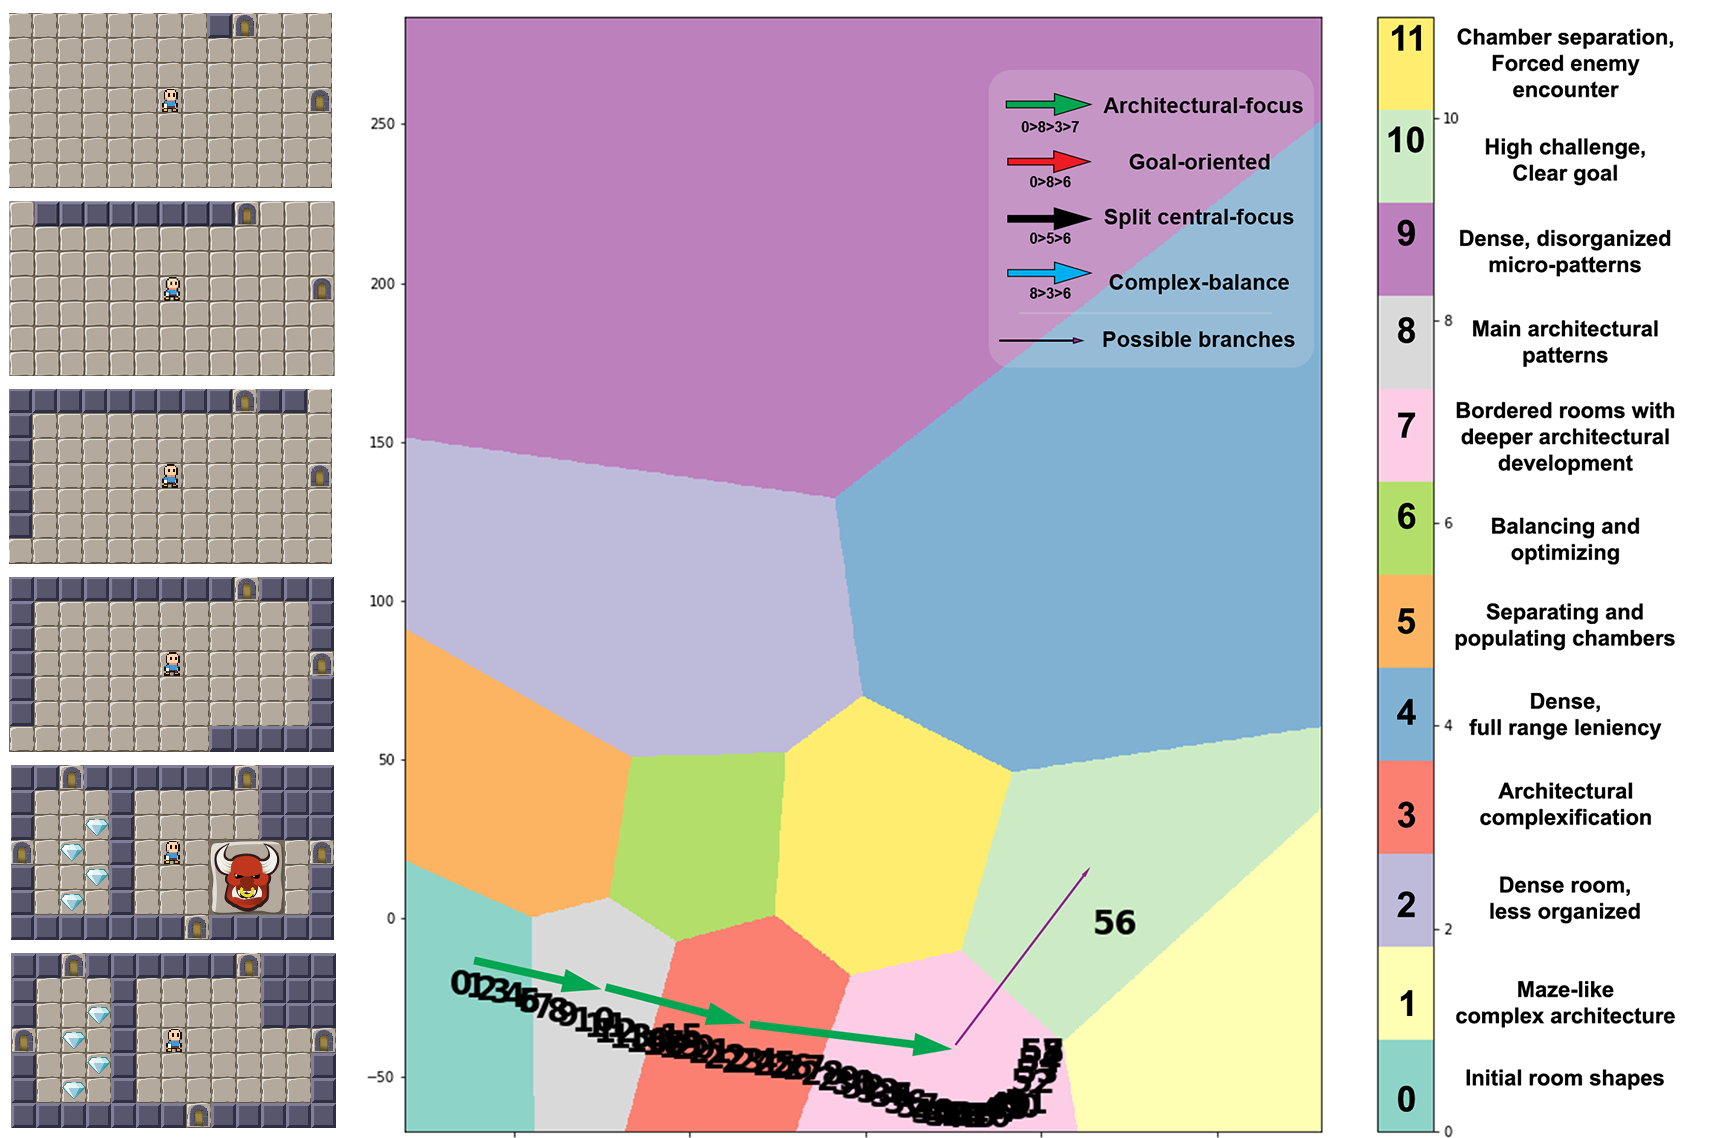
\includegraphics[width=0.95\textwidth]{figures/1.png}
%         \caption{Linearity-\#MesoPatterns}
%     \end{subfigure}%
%     \begin{subfigure}[t]{0.33\textwidth}
%         \centering
%         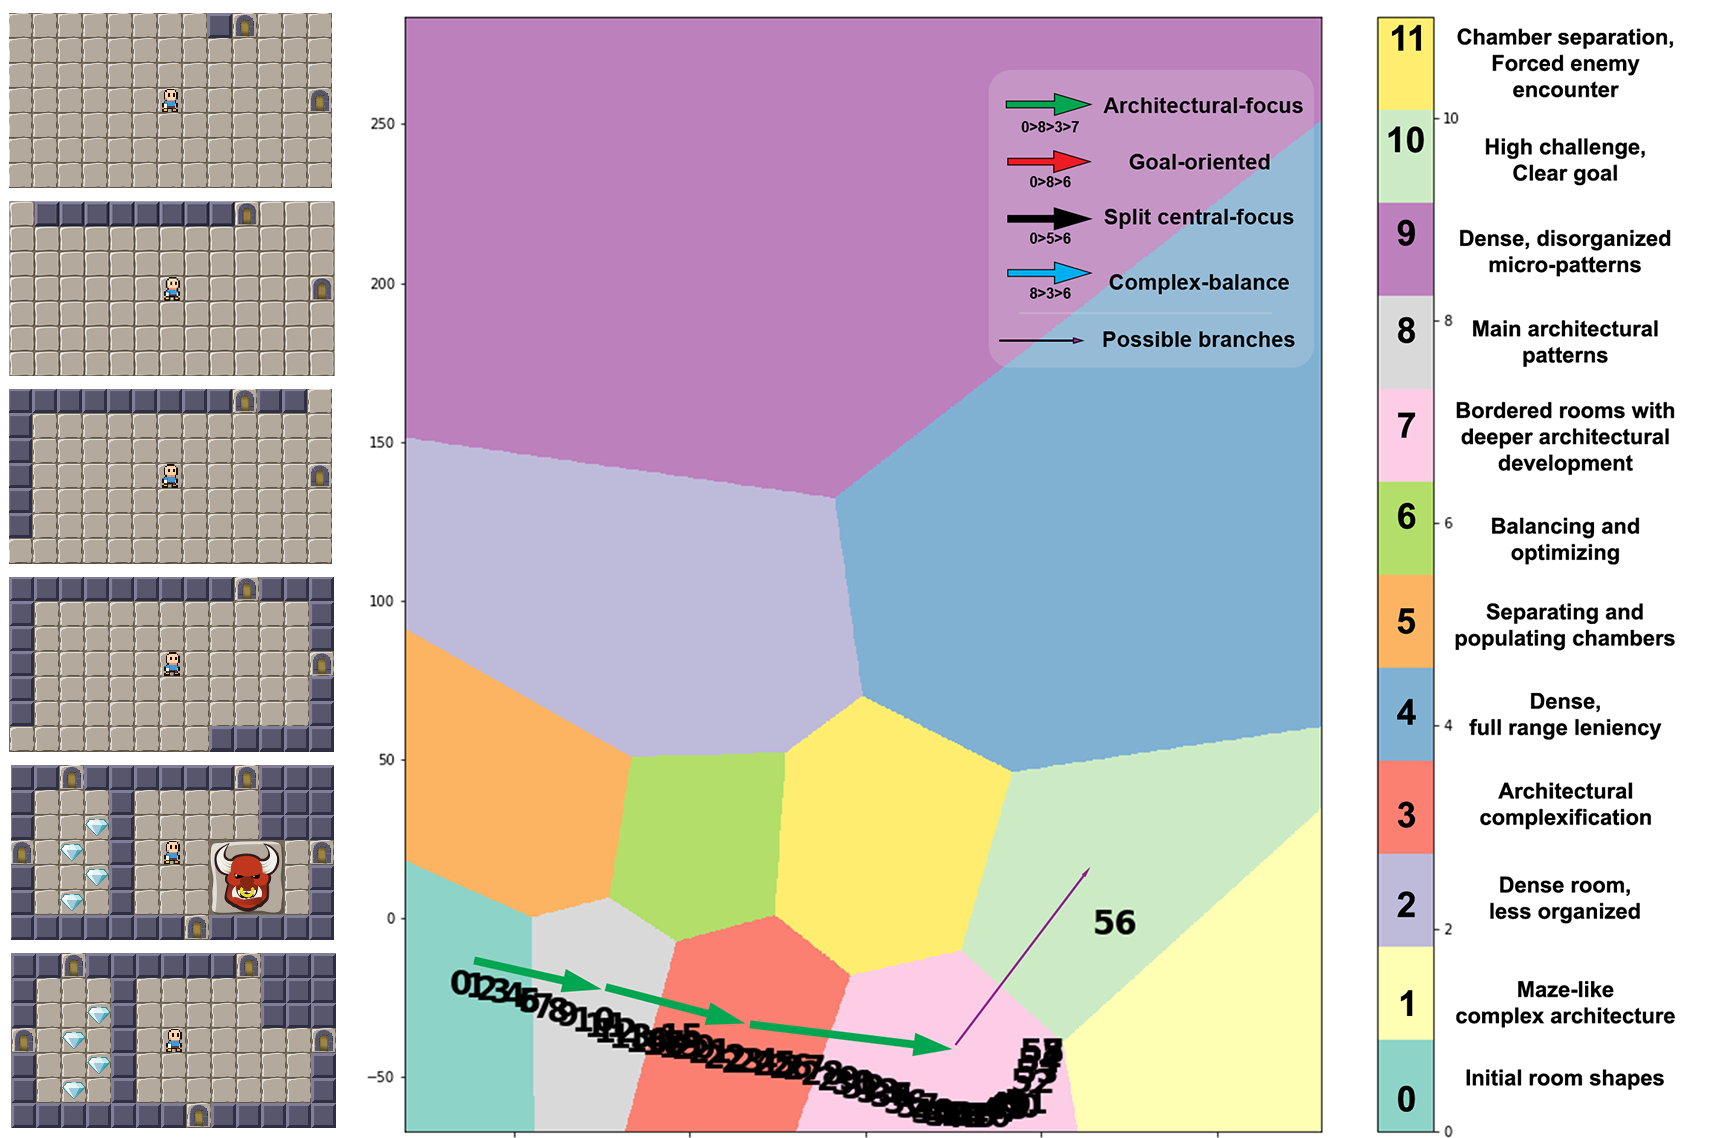
\includegraphics[width=0.95\textwidth]{figures/1.png}
%         \caption{Linearity-\#MesoPatterns}
%     \end{subfigure}%

%From the figure, it can be observed that most of the paths end or go through the "light green" and "light blue" clusters. Both relate to rooms that have a more clear structural pattern and more explicit mix between corridors and small chambers, thus, is understandable since the rooms in those clusters are or shaped as end rooms or structurally shaped to be “optimized” to a specific goal (E.g. dense bordered room, maze-like, more challenging, etc.). Further, most of the sequences end up


%Most of the rooms end there, 64 end in cluster 6 (light blue) and 52 end in cluster 11 (light green), so it makes sense that they are key steps in most of the subsequences. Further, most of the rooms start in cluster 0 (red) – 95 rooms – or in cluster 8 (purple) – 49 rooms, which make them key steps as well

%Most of the sequences with $95$ out of the $180$ starting in the red cluster, and $49$ out of the $180$ starting in the purple cluster. which correlates to the type of designs encountered in those clusters, mainly emptier rooms with initial sketches and shapes. 


%Info about the trajectories, 1) variation (length), 2) starting cluster, 3) end-point cluster.


% \begin{itemize}
%     \item[\textbf{DONE:}] Present 3 representative examples where we cluster each step of the design process. Perhaps I should create a room that would go through all the clusters?
%     \item[\textbf{DONE:}] Explain that we did this for all the 180 designs, and we collected the unique trajectories along the clusters, reducing the dimensionality of each step to each cluster.
%     \item[\textbf{DONE:}] Due to border designs (step that are in the border between 2 different clusters), we applied a threshold to reduce the noise those inputs could have when clustering the trajectories of the designer.
%     \item[\textbf{DONE:}] this data (the sequences) were then applied the GSP algorithm, a subsequence frequent pattern mining algorithm, to extract the frequent patterns in the sequences (including subsequences within the sequence).
%     \item This resulted in the following trajectories, which can also be observed in Figure X.
%     \item 
% \end{itemize}

\subsection{Conclusions}



% \begin{itemize}
%     \item Discussion on what does this archetypical design trajectories mean?
%     \item how to use them? next steps into integrating this into a system. To use this in a search-based approach as objectives for the generation to move towards the directions where (according to our archetypical design trajectories) the designers will move towards in their design process. Perhaps I could also bring the discussion from the workshop-paper for HC-AI.
%     \item discussion on creativity? is the output or the process where the actual creativity is outputted? Compare using end-design clustering to using sequences to cluster.
%     \item Discussion on how PCGRL relates to this type of work? --> Perhaps this is something for the background instead.
% \end{itemize}{}


% This paper presents a step towards designer modelling in a MI-CC environment by providing an implementation of designer personas as archetypical trajectories through style space, as a means to characterize several representative and frequent design styles together. 

%This paper presents a novel approach and meaningful steps towards designer modeling in an MI-CC environment. By providing an implementation of designer personas as archetypical trajectories through style space, we show that 

This paper presents a novel approach and meaningful steps towards designer modeling through an experiment on archetypical design trajectories analysis in an MI-CC environment. Through this, we characterize several representative design styles as designer personas. We have first run and compared several clustering setups to find the best partitioning of the design style using the edition sequences of the collected $180$ unique rooms, ending in $8196$ data points, and resulting in a set of twelve cohesive, coherent, and meaningful clusters. We have then mapped these $180$ design sequences in terms of these clusters, applying frequent sequence mining to find four frequent and unique designer styles, with related common sub-styles. As a result, we have presented a roadmap of design styles over a map of data-driven design clusters. 

%This paper presents a step towards designer modeling through an experiment on archetypical design trajectories analysis in an MI-CC environment, as a means to characterize several representative design styles as designer personas. We have first run and compared several clustering setups to find the best partitioning using the edition sequences of the collected $180$ unique rooms, ending in $8196$ data points, and resulting in a set of twelve cohesive, coherent, and meaningful clusters. We have then mapped these $180$ design sequences in terms of these clusters, applying frequent sequence mining to find four frequent unique designer styles, with related common sub-styles. As a result, we have presented a roadmap of design styles over a map of data-driven design clusters. %The examples in Figure \ref{p6fig:archetypical-examples}, help us to clarify 

%  namely the \textsc{Designer Personas}

% Our work draws on the ideas, concepts, and goals and concepts proposed by Liapis et al. when introducing the Designer Modeling as a model to capture multiple designer's processes. A prototype of such was implemented in the sentient sketchbook~\citepsixth{p6Liapis2014-designerModelImpl}, where it is proposed the use of interactive evolution by biasing the search space in favor of hand-crafted features of the design. we propose an alternative and novel route to designer modeling through clustering the design space and the room style based on the collected data. Moreover, we differ as well on the type of level design, being the sentient sketchbook a tool for strategy games~\citepsixth{p6liapis_generating_2013}, while EDD a tool for adventure and rogue-like games~\citepsixth{p6Alvarez2020-ICMAPE}. These differences strengthen the importance and usefulness of designer modeling, and highlight the holistic and generic properties of this designer-centric perspective.

Designer modeling was proposed as an approach to capture multiple designer's processes to create a better workflow by Liapis et al.~\citepsixth{p6Liapis2013-designerModel}, and our work draws on many of their ideas, concepts, and goals. Furthermore, a prototype of such was implemented in the sentient sketchbook~\citepsixth{p6Liapis2014-designerModelImpl}, where it is proposed different approaches to model style, process, and goals based on choice-based evolution and the designer's current design to adapt the provided suggestions accordingly. We propose an alternative route to designer modeling through clustering the design space and the room style based on the collected data. Moreover, we differ in the type of level design, being the sentient sketchbook a tool for strategy games~\citepsixth{p6liapis_generating_2013}, while EDD is a tool for adventure and rogue-like games~\citepsixth{p6Alvarez2020-ICMAPE}. These differences strengthen the importance and usefulness of designer modeling and highlight the holistic and generic properties of this designer-centric perspective and its possibilities.

% Designer modeling in computer-aided design tools was proposed by Liapis et al.~\citepsixth{p6Liapis2013-designerModel} as an approach to capture multiple designer's processes to create a better workflow, and a prototype of such was implemented in the sentient sketchbook~\citepsixth{p6Liapis2014-designerModelImpl}. While our work drags on many of the concepts, ideas, and goals described by Liapis et al., we propose an alternative route to designer modeling through clustering the design space

% In their work, they propose the use of hand-crafted

% Our work drags on many of the concepts, ideas, and goals described in~\citepsixth{p6Liapis2013-designerModel}, but we propose an alternative route to designer modeling through clustering the design space and the room style based on the collected data. In contrast 

% Their work propose the use of interactive evolution by biasing the search space in favor of hand-crafted features of the design akin to~\citepsixth{p6Alvarez2020-DesignerPreference}. However, we propose an alternative and novel route to designer modeling through clustering the design space and the room style based on the collected data. Moreover, we differ as well on the type of level design, being the sentient sketchbook a tool for strategy games~\citepsixth{p6liapis_generating_2013}, while EDD a tool for adventure and rogue-like games~\citepsixth{p6Alvarez2020-ICMAPE}. Applying the idea of designer modelling to both genres, not only shows the importance and usefulness of designer modeling but also the holistic and generic view 

% These differences strengthen the importance and usefulness of designer modeling, and highlight the holistic and generic properties of this designer-centric perspective.

% % might be interesting to discuss this.
% While the approach described in this paper is applied in a tool for creating zelda-like dungeon games~\citepsixth{p6tloz}, the approach can be reused and extended to other domains 

These contributions allow us to better understand, cluster, categorize and isolate designer behavior. This is very valuable for mixed-initiative approaches, where a clear virtual model of the designer's style allows us to better drive the search process for procedurally generating content that is valuable for the designer. Designer personas have the potential to be used in many different scenarios. For instance, as objectives for a search-based approach to enable a more style-sensitive system, to evaluate the fitness of evolutionary generated content or to train PCG agents via Reinforcement Learning~\citepsixth{p6khalifa2020-pcgrl}. 

Moreover, recognizing the designers' current style and the path taken so far, which would indicate a possible designer persona, could open the possibility for recognizing their intentions, preferences, and goals. This traced roadmap of designer personas could let a content generator anticipate a designer's next moves without heavy computational cost, just by identifying her current location on the map and offering content suggestions that lie in the most promising clusters to be visited next. Conversely, it could also identify designers who do not follow a certain path, i.e. deviating from the pattern, trying to understand their objective through their design style.

% Finally, in our work, we did not observe any type of cross-path i.e. a design going from one path to another. We believe that this is due to the level at which we observe the archetypical paths. However, preliminary analysis on the dataset used in this paper and as expected, the design process of designed rooms within the same dungeon does follow different paths, and sometimes even crossing each other. This opens an interesting and exciting area to explore a wider layer, taking rooms as a set of archetypical paths taken by designers. Observing the paths taken in previous and future rooms, and the dungeon as a whole, as briefly introduced in section~\ref{p6sec:designStyle}, to understand the designers' intentions and goals when they proceed to create a new room is a promising future step to take with the current system. 

%  i.e. room-wise, as the designer typically would design the room with a set of goals

Finally, it is also important to observe the nature of the previous and future rooms created by a designer. Observing the dungeon as a whole, as briefly introduced in section~\ref{p6sec:designStyle}, to understand the designers' intentions and goals when they proceed to create a new room is a promising future step to take with the current system. 

% Furthermore, the designer personas addresses the dynamic-dynamic system vs. dynamic-static system open question raised by Alvarez and Font~\citepsixth{p6Alvarez2020-DesignerPreference}, which relates to the challenge of adapting a system to the a ever-changing designer. With the use of the archetypical paths, the model is not anymore adapting and moving through the solution space with the designer, rather the designer traverse through an already clustered space. 

% With the use of the archetypical paths, we can not only identify the current designer persona the designer is following but we can also adapt and anticipate to what they might end up doing. 

% Furthermore, the designer personas addresses an open question raised by Alvarez and Font \citepsixth{p6Alvarez2020-DesignerPreference}, related to the challenges  using a dynamic-dynamic system vs. a dynamic-static system. The authors describe the dynamic-dynamic system as a system where both designer and AI-system move through the solution space, with the AI-system constantly trying to adapt to the designer. They concluded that the main challenge correspond to designers constantly concept drifting resulting in them continuously changing their decisions. Instead, the authors proposed the use of a dynamic-static system, where the model is not anymore adapting and moving through the solution space with the designer, rather the designer traverse through an already clustered space. With the use of the archetypical paths, we can not only identify the current designer persona the designer is following but we can also adapt and anticipate to what they might end up doing. 


%and conclude that the main challenges in

% Moreover, this traced roadmap of designer personas could let a content generator anticipate a designer's next moves without heavy computational cost, just by identifying her current location on the map and offering content suggestions that lie in the most promising clusters to be visited next. %Further, one could also be able to identify designers that do not follow a certain path i.e. deviating from the pattern, and try to understand through their design style their objective.





% From the $180$ unique rooms, we extracted and used the edition sequence of each of the rooms, from their initial design to the more elaborated end-design, to compose a richer dataset that could capture the design process of a designer rather than focusing on the end-point. Through this, we ended up using $8196$ data points in our dataset.

% We have first run and compared s


% through experimenting with 

% This paper presents a step towards designer modelling by providing a prototype implementation of designer personas as archetypical trajectories through style space. These archetypical paths

% This paper presents an experiment on archetypical design trajectories analysis in a MI-CC environment, as a means to characterize several representative design styles as designer personas. We have first run and compared several clustering setups to find the best partitioning, resulting into a set of twelve cohesive, coherent, and meaningful clusters. We have then mapped almost 200 complete design sequences in terms of these clusters, applying sequence mining to find four frequent unique designer styles, with related common sub-styles. As a result, we have presented a roadmap of design styles over a map of data-driven design clusters. 



% be used as goal for other systems were anticipating a design or creating a synthetic objective might be more complicated. We envision that these designer personas can be used within 

\bibliographystylepeleventh{ieeetr}
\bibliographypeleventh{included-papers-tex/paper-11/references.bib}